\documentclass[11pt]{article}
\usepackage[margin=1in]{geometry}
\usepackage[T1]{fontenc}
\usepackage{mathptmx}
\usepackage{setspace}\setstretch{1.08}
\usepackage{graphicx,booktabs,amsmath,amssymb,amsthm,xspace,caption,longtable,listings,float,array}
\usepackage[hidelinks]{hyperref}
\usepackage{natbib}\bibpunct{(}{)}{;}{a}{}{,}
\captionsetup{font=small,labelfont=bf}
\renewcommand{\thetable}{A\arabic{table}}\renewcommand{\thefigure}{A\arabic{figure}}
\newtheorem{theorem}{Theorem}\newtheorem{corollary}{Corollary}\newtheorem{assumption}{Assumption}
\theoremstyle{remark}\newtheorem{remark}{Remark}
\lstset{basicstyle=\ttfamily\scriptsize,breaklines=true,columns=fullflexible,frame=single}
\xspaceaddexceptions{\%}
% generated by scripts/17_numbers.py -- do not edit
\newcommand{\NfirmYears}{34,333\xspace}
\newcommand{\Nfirms}{4,078\xspace}
\newcommand{\NlinkedFirms}{11,182\xspace}
\newcommand{\CorrHeadcount}{0.89\xspace}
\newcommand{\GitHubValid}{2.6\xspace}
\newcommand{\HFValid}{20\xspace}
\newcommand{\GenAIrows}{3.9\xspace}
\newcommand{\HoneB}{1.21\xspace}
\newcommand{\HoneT}{9.7\xspace}
\newcommand{\HonePct}{3.3\xspace}
\newcommand{\HoneIndB}{0.74\xspace}
\newcommand{\HoneIndT}{3.2\xspace}
\newcommand{\EntryAloneB}{-0.28\xspace}
\newcommand{\EntryAloneT}{-3.3\xspace}
\newcommand{\EntryAloneAbs}{0.28\xspace}
\newcommand{\PkgHoneB}{-1.08\xspace}
\newcommand{\PkgHoneT}{10.6\xspace}
\newcommand{\PkgHoneAbs}{1.08\xspace}
\newcommand{\PkgPyrB}{-0.35\xspace}
\newcommand{\PkgPyrT}{5.6\xspace}
\newcommand{\PkgRemB}{-0.31\xspace}
\newcommand{\PkgRemT}{4.6\xspace}
\newcommand{\PkgAgeB}{0.13\xspace}
\newcommand{\PkgAgeT}{2.6\xspace}
\newcommand{\PyrHi}{13.5\xspace}
\newcommand{\PyrLo}{6.9\xspace}
\newcommand{\RemHi}{13.2\xspace}
\newcommand{\RemLo}{7.3\xspace}
\newcommand{\AgeHi}{9.0\xspace}
\newcommand{\AgeLo}{11.5\xspace}
\newcommand{\FSF}{562\xspace}
\newcommand{\FSB}{0.18\xspace}
\newcommand{\IVtiltB}{6.5\xspace}
\newcommand{\IVtiltSE}{0.7\xspace}
\newcommand{\PretrendP}{0.011\xspace}
\newcommand{\Mbar}{1.5\xspace}
\newcommand{\TrendB}{1.38\xspace}
\newcommand{\TrendBT}{10.2\xspace}
\newcommand{\LateB}{1.26\xspace}
\newcommand{\LateBT}{10.2\xspace}
\newcommand{\NegCtl}{-0.44\xspace}
\newcommand{\NegCtlT}{3.6\xspace}
\newcommand{\PlaceboNineteen}{-0.26\xspace}
\newcommand{\PlaceboNineteenT}{2.7\xspace}
\newcommand{\EvTwentyThree}{1.25\xspace}
\newcommand{\EvTwentyFive}{1.80\xspace}
\newcommand{\ModelsToFirstU}{3,483\xspace}
\newcommand{\ModelsU}{4,156\xspace}
\newcommand{\ModelsToFirstFree}{12\xspace}
\newcommand{\ShareHoneSig}{54\xspace}
\newcommand{\HoneMaxT}{12.1\xspace}
\newcommand{\NbaseSpecs}{648\xspace}
\newcommand{\BonfCrit}{4.2\xspace}
\newcommand{\GuardExploreSuccess}{no\xspace}
\newcommand{\GuardConfHoneT}{7.4\xspace}
\newcommand{\Bnull}{1,000\xspace}
\newcommand{\PotemU}{26.5\xspace}
\newcommand{\PotemFree}{93.4\xspace}
\newcommand{\PotemBonf}{0.0\xspace}
\newcommand{\PotemSpec}{3.3\xspace}
\newcommand{\PotemNWC}{5.0\xspace}
\newcommand{\PotemGuard}{0.6\xspace}
\newcommand{\BGuard}{500\xspace}
\newcommand{\GuardHonePot}{48\xspace}
\newcommand{\pNWChOne}{0.001\xspace}
\newcommand{\pNWCpkg}{0.056\xspace}
\newcommand{\NullHoneQ}{8.6\xspace}
\newcommand{\NullHoneMed}{7.4\xspace}
\newcommand{\BonfHoneCrit}{3.8\xspace}
\newcommand{\BonfHonePot}{100\xspace}
\newcommand{\NullShareHoneSig}{34\xspace}
\newcommand{\pBPyr}{0.002\xspace}
\newcommand{\BBPyr}{500\xspace}
\newcommand{\SelPyr}{0.4\xspace}
\newcommand{\HolmPyr}{0.006\xspace}
\newcommand{\pBRem}{0.046\xspace}
\newcommand{\BBRem}{500\xspace}
\newcommand{\SelRem}{92.8\xspace}
\newcommand{\HolmRem}{0.092\xspace}
\newcommand{\pBAge}{0.313\xspace}
\newcommand{\BBAge}{500\xspace}
\newcommand{\SelAge}{76.6\xspace}
\newcommand{\HolmAge}{0.313\xspace}
\newcommand{\PlantPowerLow}{98\xspace}
\newcommand{\PlantPowerMid}{98\xspace}
\newcommand{\PlantPowerHigh}{98\xspace}
\newcommand{\PlantPowerBonf}{93\xspace}
\newcommand{\PlantPowerU}{100\xspace}
\newcommand{\WinnerCurse}{3.2\xspace}
\newcommand{\MCsizeNWC}{5.0\xspace}
\newcommand{\MCsizeNWCpkg}{0.0\xspace}
\newcommand{\MCsizeU}{0.0\xspace}
\newcommand{\MCsizeSpec}{11.0\xspace}
\newcommand{\MCsizeLeak}{10.3\xspace}
\newcommand{\MCsizeLeakReplay}{5.0\xspace}
\newcommand{\MCsizeConf}{90.0\xspace}
\newcommand{\MCpowerNWChOne}{100.0\xspace}
\newcommand{\MCpowerNWC}{82.0\xspace}
\newcommand{\MCpowerU}{82.0\xspace}
\newcommand{\MCR}{300\xspace}
\newcommand{\MCB}{39\xspace}
\newcommand{\RegistryHash}{9aec7d8707aa63a2\xspace}
\newcommand{\RegistryTime}{2026-09-29 04:19:18 BST\xspace}

% generated by scripts/25_aggregate_validity.py -- do not edit
\newcommand{\VSelPyr}{0.4\xspace}
\newcommand{\VNselPyr}{2\xspace}
\newcommand{\VpSelPyr}{0.002\xspace}
\newcommand{\VpFreePyr}{0.002\xspace}
\newcommand{\VpFixPyr}{0.002\xspace}
\newcommand{\VFreeObsPyr}{6.3\xspace}
\newcommand{\VpResSelPyr}{0.002\xspace}
\newcommand{\VpResFreePyr}{0.002\xspace}
\newcommand{\VpResFixPyr}{0.002\xspace}
\newcommand{\VResHolmTenPyr}{0.020\xspace}
\newcommand{\VpFLSelPyr}{0.002\xspace}
\newcommand{\VpFLFreePyr}{0.002\xspace}
\newcommand{\VpFLFixPyr}{0.002\xspace}
\newcommand{\VFLHolmTenPyr}{0.020\xspace}
\newcommand{\VHolmThreePyr}{0.006\xspace}
\newcommand{\VHolmTenPyr}{0.020\xspace}
\newcommand{\VMinPPyr}{0.010\xspace}
\newcommand{\VMaxTPyr}{0.171\xspace}
\newcommand{\VMinPFreePyr}{0.009\xspace}
\newcommand{\VSelRem}{92.8\xspace}
\newcommand{\VNselRem}{464\xspace}
\newcommand{\VpSelRem}{0.046\xspace}
\newcommand{\VpFreeRem}{0.601\xspace}
\newcommand{\VpFixRem}{0.018\xspace}
\newcommand{\VFreeObsRem}{14.8\xspace}
\newcommand{\VpResSelRem}{0.054\xspace}
\newcommand{\VpResFreeRem}{0.337\xspace}
\newcommand{\VpResFixRem}{0.058\xspace}
\newcommand{\VResHolmTenRem}{0.485\xspace}
\newcommand{\VpFLSelRem}{0.032\xspace}
\newcommand{\VpFLFreeRem}{0.693\xspace}
\newcommand{\VpFLFixRem}{0.184\xspace}
\newcommand{\VFLHolmTenRem}{0.287\xspace}
\newcommand{\VHolmThreeRem}{0.092\xspace}
\newcommand{\VHolmTenRem}{0.413\xspace}
\newcommand{\VMinPRem}{0.678\xspace}
\newcommand{\VMaxTRem}{0.279\xspace}
\newcommand{\VMinPFreeRem}{0.979\xspace}
\newcommand{\VSelAge}{76.6\xspace}
\newcommand{\VNselAge}{383\xspace}
\newcommand{\VpSelAge}{0.313\xspace}
\newcommand{\VpFreeAge}{0.002\xspace}
\newcommand{\VpFixAge}{0.022\xspace}
\newcommand{\VFreeObsAge}{7.0\xspace}
\newcommand{\VpResSelAge}{0.234\xspace}
\newcommand{\VpResFreeAge}{0.004\xspace}
\newcommand{\VpResFixAge}{0.228\xspace}
\newcommand{\VResHolmTenAge}{1.000\xspace}
\newcommand{\VpFLSelAge}{0.365\xspace}
\newcommand{\VpFLFreeAge}{0.220\xspace}
\newcommand{\VpFLFixAge}{0.146\xspace}
\newcommand{\VFLHolmTenAge}{1.000\xspace}
\newcommand{\VHolmThreeAge}{0.313\xspace}
\newcommand{\VHolmTenAge}{1.000\xspace}
\newcommand{\VMinPAge}{0.678\xspace}
\newcommand{\VMaxTAge}{0.651\xspace}
\newcommand{\VMinPFreeAge}{0.009\xspace}
\newcommand{\VBjoint}{1,000\xspace}
\newcommand{\VJointSuccess}{94.0\xspace}
\newcommand{\VFwerUnadj}{34.9\xspace}
\newcommand{\VFwerHolmThree}{14.4\xspace}
\newcommand{\VFwerHolmTen}{4.7\xspace}
\newcommand{\VBcovA}{1,000\xspace}
\newcommand{\VcovAph}{0.001\xspace}
\newcommand{\VcovApkg}{0.137\xspace}
\newcommand{\VcovAPotU}{40.3\xspace}
\newcommand{\VcovAPotFree}{100.0\xspace}
\newcommand{\VcovAhQ}{8.0\xspace}
\newcommand{\VcovAhMax}{9.3\xspace}
\newcommand{\VcovARsq}{53\xspace}
\newcommand{\VTypeAhMax}{9.8\xspace}
\newcommand{\VcorrExpRem}{0.62\xspace}
\newcommand{\VcorrExpPyr}{$-$0.53\xspace}
\newcommand{\VcorrExpAI}{0.49\xspace}
\newcommand{\VcorrExpGrowth}{0.16\xspace}
\newcommand{\VcorrPyrRemCell}{$-$0.38\xspace}
\newcommand{\VcorrPyrWageCell}{$-$0.33\xspace}
\newcommand{\VcorrPyrIlmCell}{0.26\xspace}
\newcommand{\VpTmax}{0.124\xspace}
\newcommand{\VSecWorld}{2.5\xspace}
\newcommand{\VSpeedup}{72\xspace}
\newcommand{\VFitsWorld}{5,647\xspace}
\newcommand{\VPyfixestWorld}{182\xspace}
\newcommand{\VPyfixestModel}{0.032\xspace}
\newcommand{\VNhPass}{347\xspace}
\newcommand{\VExSingleNull}{17.0\xspace}
\newcommand{\VExNaiveNull}{19.5\xspace}
\newcommand{\VBudUThousand}{3.7\xspace}
\newcommand{\VBudUReal}{25.7\xspace}
\newcommand{\VBudFreeTwelve}{8.3\xspace}
\newcommand{\VBudFreeHundred}{23.5\xspace}
\newcommand{\VBudUTwelve}{0.9\xspace}
\newcommand{\VModelsMin}{2,169\xspace}
\newcommand{\VModelsMax}{5,171\xspace}
\newcommand{\VModelsMed}{2,790\xspace}
\newcommand{\VTriples}{21\xspace}
\newcommand{\VBaseDistinct}{53\xspace}
\newcommand{\VExNull}{6.5\xspace}
\newcommand{\VExLevel}{6.0\xspace}
\newcommand{\VExCovMax}{7.5\xspace}
\newcommand{\VExStratMax}{45.0\xspace}
\newcommand{\VExNcells}{12\xspace}
\newcommand{\VExNWCSixTen}{100.0\xspace}
\newcommand{\VExSingleSixTen}{84.5\xspace}
\newcommand{\VExNaiveSixTen}{87.0\xspace}
\newcommand{\VExCovSixTen}{5.5\xspace}
\newcommand{\VExStratSixTen}{19.5\xspace}
\newcommand{\VExSpurSixTen}{26\xspace}
\newcommand{\VExNWCSixTwenty}{100.0\xspace}
\newcommand{\VExSingleSixTwenty}{100.0\xspace}
\newcommand{\VExNaiveSixTwenty}{100.0\xspace}
\newcommand{\VExCovSixTwenty}{4.5\xspace}
\newcommand{\VExStratSixTwenty}{45.0\xspace}
\newcommand{\VExSpurSixTwenty}{51\xspace}
\newcommand{\VExNWCTwoQuarter}{11.5\xspace}
\newcommand{\VExSingleTwoQuarter}{20.0\xspace}
\newcommand{\VExNaiveTwoQuarter}{23.5\xspace}
\newcommand{\VExCovTwoQuarter}{6.5\xspace}
\newcommand{\VExStratTwoQuarter}{6.0\xspace}
\newcommand{\VExSpurTwoQuarter}{3\xspace}
\newcommand{\VExNWCFourFive}{43.0\xspace}
\newcommand{\VExSingleFourFive}{35.0\xspace}
\newcommand{\VExNaiveFourFive}{43.0\xspace}
\newcommand{\VExCovFourFive}{7.0\xspace}
\newcommand{\VExStratFourFive}{8.0\xspace}
\newcommand{\VExSpurFourFive}{9\xspace}
\newcommand{\VExNWCTwoFive}{19.5\xspace}
\newcommand{\VExSingleTwoFive}{25.0\xspace}
\newcommand{\VExNaiveTwoFive}{30.0\xspace}
\newcommand{\VExCovTwoFive}{7.0\xspace}
\newcommand{\VExStratTwoFive}{6.0\xspace}
\newcommand{\VExSpurTwoFive}{5\xspace}
\newcommand{\VMmPermFreeClean}{4.0\xspace}
\newcommand{\VMmPermFixClean}{4.0\xspace}
\newcommand{\VMmResFreeClean}{7.0\xspace}
\newcommand{\VMmResFixClean}{5.0\xspace}
\newcommand{\VMmFLFreeClean}{0.5\xspace}
\newcommand{\VMmFLFixClean}{0.5\xspace}
\newcommand{\VMmNomFixClean}{2.5\xspace}
\newcommand{\VMmNomFreeClean}{4.5\xspace}
\newcommand{\VMmPermFreeTrend}{1.5\xspace}
\newcommand{\VMmPermFixTrend}{2.0\xspace}
\newcommand{\VMmResFreeTrend}{5.5\xspace}
\newcommand{\VMmResFixTrend}{5.0\xspace}
\newcommand{\VMmFLFreeTrend}{1.0\xspace}
\newcommand{\VMmFLFixTrend}{0.5\xspace}
\newcommand{\VMmNomFixTrend}{2.5\xspace}
\newcommand{\VMmNomFreeTrend}{3.5\xspace}
\newcommand{\VMmPermFreeProxy}{65.5\xspace}
\newcommand{\VMmPermFixProxy}{67.5\xspace}
\newcommand{\VMmResFreeProxy}{5.0\xspace}
\newcommand{\VMmResFixProxy}{5.0\xspace}
\newcommand{\VMmFLFreeProxy}{0.5\xspace}
\newcommand{\VMmFLFixProxy}{0.5\xspace}
\newcommand{\VMmNomFixProxy}{95.0\xspace}
\newcommand{\VMmNomFreeProxy}{96.0\xspace}
\newcommand{\VMmPermFreeNonlin}{35.5\xspace}
\newcommand{\VMmPermFixNonlin}{35.0\xspace}
\newcommand{\VMmResFreeNonlin}{5.5\xspace}
\newcommand{\VMmResFixNonlin}{6.0\xspace}
\newcommand{\VMmFLFreeNonlin}{0.5\xspace}
\newcommand{\VMmFLFixNonlin}{0.5\xspace}
\newcommand{\VMmNomFixNonlin}{96.0\xspace}
\newcommand{\VMmNomFreeNonlin}{96.5\xspace}
\newcommand{\VMmPermFreeAll}{91.5\xspace}
\newcommand{\VMmPermFixAll}{95.0\xspace}
\newcommand{\VMmResFreeAll}{4.5\xspace}
\newcommand{\VMmResFixAll}{4.5\xspace}
\newcommand{\VMmFLFreeAll}{0.5\xspace}
\newcommand{\VMmFLFixAll}{0.5\xspace}
\newcommand{\VMmNomFixAll}{100.0\xspace}
\newcommand{\VMmNomFreeAll}{96.5\xspace}


\title{\textbf{Technical Appendix}\\[2pt]\large Potemkin Findings: Calibrating AI Research Loops with Null Worlds}
\date{}
\begin{document}
\maketitle
\tableofcontents
\clearpage

%======================================================================
\section{Formal framework and validity of loop-level inference}\label{sec:theory}
%======================================================================

\subsection{Objects}
Let firms $i=1,\dots,N$ be partitioned into strata $g(i)$. The data are $D=(Y,E,M,X,g)$:
\begin{itemize}
\item $Y$ is the panel of outcomes;
\item $E=(E_1,\dots,E_N)$ is the firm-level treatment (possibly several proxies per firm);
\item $M$ is the firm-level moderators;
\item $X$ is the panel of controls.
\end{itemize}
A \emph{design space} $S$ is a finite set of specifications. Each specification is a tuple (outcome proxy, treatment proxy,
control set, fixed-effect structure, sample rule, transformation, clustering, moderator subset).

A \emph{search policy} $\pi$ is a deterministic rule that:
\begin{itemize}
\item visits specifications in an order that may depend on results already seen;
\item stops by a rule that may also depend on those results;
\item returns a report $R$.
\end{itemize}
The \emph{loop} is the map $L_{S,\pi}:D\mapsto R$, and $T(R)$ is a real-valued evidence statistic of the report. In this
paper $T$ is either the largest sign-consistent H1 $t$-statistic visited or the smallest sign-consistent $t$-statistic
among the four hypotheses in the reported package.

For a permutation $\sigma$ of firm labels, $D^{\sigma}=(Y,E\circ\sigma,M,X,g)$ reassigns each firm the treatment of firm
$\sigma(i)$ and leaves everything else unchanged. Let $\mathcal G$ be the group of permutations that map each stratum onto
itself.

\begin{assumption}[Within-stratum exchangeability under the null]\label{ass:exch}
Under $H_0$, $D^{\sigma}\overset{d}{=}D$ for every $\sigma\in\mathcal G$.
\end{assumption}

Assumption~\ref{ass:exch} holds, for example, when outcomes, moderators, and controls do not depend on the treatment (the
sharp null) and the treatment is assigned exchangeably within strata. In observational data it is a design-based
assumption. It is stronger than the conditional parallel-trends assumption behind the difference-in-differences estimates
in Section~\ref{sec:testbed}. Null-World Calibration therefore prices \emph{search}; it does not by itself establish
causality.

\begin{theorem}[Validity of loop-level randomization inference]\label{thm:valid}
Let $L$ be any deterministic loop whose design space $S$ and policy $\pi$ are fixed independently of the realized data,
and let $T$ be any real-valued statistic of its report. Draw $\sigma_1,\dots,\sigma_B$ independently and uniformly from
$\mathcal G$, independently of $D$. Define
\[
p_L=\frac{1+\sum_{b=1}^{B}\mathbb 1\{T(L(D^{\sigma_b}))\ge T(L(D))\}}{B+1}.
\]
Under Assumption~\ref{ass:exch}, $\Pr(p_L\le\alpha)\le\alpha$ for every $\alpha\in(0,1)$ and every $B\ge1$.
\end{theorem}

\begin{proof}
Write $V(D)=T(L(D))$. Because $L$ and $T$ are fixed functions, $V$ is a fixed measurable function of the data.

\emph{Step 1: the $B+1$ datasets are exchangeable.} Let $\rho$ be uniform on $\mathcal G$, independent of $D$ and of
$(\sigma_b)$. By Assumption~\ref{ass:exch}, $D\overset{d}{=}D^{\rho}$. Applying the map
$D\mapsto(D,D^{\sigma_1},\dots,D^{\sigma_B})$ to both sides gives
\[
(D,D^{\sigma_1},\dots,D^{\sigma_B})\overset{d}{=}(D^{\rho},D^{\sigma_1\rho},\dots,D^{\sigma_B\rho}).
\]
Because $\mathcal G$ is a group and $\sigma_b$ is uniform and independent of $\rho$, the elements
$\rho,\sigma_1\rho,\dots,\sigma_B\rho$ are i.i.d.\ uniform on $\mathcal G$. The right-hand side is therefore an
exchangeable sequence (conditionally on $D$, and hence unconditionally). So is the left-hand side.

\emph{Step 2: the statistics are exchangeable.} Applying the fixed function $V$ coordinatewise preserves exchangeability,
so $(V_0,V_1,\dots,V_B)=(V(D),V(D^{\sigma_1}),\dots,V(D^{\sigma_B}))$ is exchangeable.

\emph{Step 3: the rank of $V_0$ is super-uniform.} For an exchangeable vector, the number $K=\#\{b\ge0: V_b\ge V_0\}$
(which counts $b=0$) satisfies $\Pr(K\le k)\le k/(B+1)$ for $k=1,\dots,B+1$. Ties only increase $K$. Since $p_L=K/(B+1)$,
$\Pr(p_L\le\alpha)=\Pr(K\le\lfloor\alpha(B+1)\rfloor)\le\lfloor\alpha(B+1)\rfloor/(B+1)\le\alpha$.
\end{proof}

\begin{remark}[What Theorem~\ref{thm:valid} adds, and what it does not]\label{rem:adds}
The argument is the classical one for randomization tests: a test is exact for any statistic fixed before the data are
seen, also when the permutations are drawn at random and the identity is counted
\citep{lehmann2022testing,hemerik2018exact}. A deterministic loop's report is such a statistic, so the theorem adds no new
statistical principle. What it adds for AI research loops is the statement of its two hypotheses in checkable form.
\begin{enumerate}
\item \emph{Completeness of the replay.} $L$ must be a fixed function of the data. Every choice that depends on outcomes
must be inside $L$, and none outside. Replayability is how this is verified, and it is necessary but not sufficient. In the
Monte Carlo, a single pruning step taken after peeking and left out of the replay doubles the size of the test
(\MCsizeLeak\% instead of \MCsizeLeakReplay\%; Section~\ref{sec:mc}).
\item \emph{Exchangeability} (Assumption~\ref{ass:exch}). The null worlds must have the distribution of the data under the
null. Section~\ref{sec:validity} measures what happens when they do not.
\end{enumerate}
Fixed-family corrections for data snooping \citep{white2000reality,romano2005stepwise,hansen2005test} rest on the same
resampling logic, but they need the family of tests enumerated in advance. An adaptive loop's family is itself random. In the
\Bnull Type~A worlds, the registered loop fits between \VModelsMin and \VModelsMax models (median \VModelsMed), and its
reported packages use \VTriples different moderator triples on \VBaseDistinct base specifications. Replay prices the path the
loop actually took. Pricing the whole registered garden instead, through the best package anywhere in the design space, is
valid but blunter: it gives $p=\VpTmax$ for the real package, against $p=\pNWCpkg$ for the loop's actual stopping rule
(\texttt{tables/benchmark.json}).
\end{remark}

\begin{remark}[What adaptivity is allowed, and what breaks validity]
The loop may search, stop, prune, rationalize signs, or select outcomes and moderators as adaptively as it likes, because
every null world is processed by the \emph{same} function. Validity breaks when some input to the report depends on $D$
through a channel that is not replayed in $D^{\sigma}$. Examples are a human or language-model decision made after seeing
results (``this moderator looks promising''), or a design space edited after an exploratory run. The registry, frozen and
hashed before outcomes were computed, is the device that rules this out. The ``leakage'' scenario of the Monte Carlo
(Section~\ref{sec:mc}) quantifies the distortion when it is violated.
\end{remark}

\begin{corollary}[Search-adjusted moderator tests]\label{cor:mod}
Fix a moderator $k$ and strata $s(i)=(g(i),q(E_i))$, where $q(\cdot)$ is the treatment quintile. Let $\mathcal G_k$ permute
the column $M_k$ within strata $s$. Suppose $D^{\sigma}\overset{d}{=}D$ for $\sigma\in\mathcal G_k$, that is, $M_k$ is
exchangeable within strata given everything else. Then the statistic $V_k(D)$ (the sign-consistent $t$ of $M_k$ in the
reported package, or $-\infty$ if $M_k$ is not reported) yields a valid $p$-value by Theorem~\ref{thm:valid}.
\end{corollary}

\paragraph{Two moderator nulls.} The permutation null of Corollary~\ref{cor:mod}, $H_{0k}^{\text{perm}}$, says that $M_k$
carries no information about outcomes within strata. It implies, but is not implied by, the hypothesis the theory states,
$H_{0k}^{\text{int}}$: the effect of exposure does not vary with $M_k$. Permuting $M_k$ also breaks its own outcome trend and its
within-stratum correlation with the other moderators (for hierarchy shape, \VcorrPyrRemCell with digitizable work inside sector
$\times$ exposure-quintile cells). A rejection of $H_{0k}^{\text{perm}}$ can therefore come from structure other than the
interaction. Firm fixed effects absorb $M_k$'s level, and every moderator model contains $M_k\times\text{Post}$, which
absorbs its linear post-shock trend in the real data. Neither term reproduces those relations in the permuted worlds.
Null-model worlds (Section~\ref{sec:worlds}) target $H_{0k}^{\text{int}}$ directly. They keep $M_k$ and all its relations
fixed and remove only the interaction. They are not exactly exchangeable: their validity is asymptotic, as for the wild
cluster bootstrap \citep{cameron2008bootstrap}, and requires the restricted model to contain the structure that the loop's
other specifications can detect. Section~\ref{sec:validity} reports their size and their $p$-values on the real data.

\paragraph{The statistic.} $V_k$ is $-\infty$ in every world in which the loop does not report $M_k$, so
\[
p_k=\Pr(\text{the loop reports }M_k\text{ and }V_k\ge v_k)
\]
combines selection and strength. Two further statistics, defined
in every world, separate them (Section~\ref{sec:validity}). $V_k^{\text{free}}$ is the largest sign-consistent
single-moderator $t$ of $M_k$ over the base specifications with a significant H1, the statistic the loop screens on.
$V_k^{\text{fix}}$ is the $t$ of $M_k$ in the reported specification with its two partner moderators, with no search. Both were
added in response to review. They are diagnostics, and no claim rests on them alone.

\paragraph{Familywise error over the ten registered moderators.} The loop reports three of ten candidates, so the family is
all ten. For an unreported candidate $V_k(D)=-\infty$ and $p_k=1$. Holm's step-down over the ten $p$-values (seven of them
equal to one) therefore controls the familywise error rate in the strong sense whenever each $p_k$ is valid, under any
dependence. It multiplies the three reported $p$-values by 10, 9, and 8. Holm over the three reported $p$-values alone carries
no such guarantee, because those three were selected for being small: the union bound runs over all ten candidates. In the
joint worlds of Section~\ref{sec:validity}, scored against one another, Holm over the three reported moderators confirms at
least one in \VFwerHolmThree\% of worlds in which none of the ten matters. Holm over ten does so in \VFwerHolmTen\%. Joint
worlds, in which all ten moderators are permuted independently within strata in the same world, give the Westfall--Young
adjustments \citep{westfall1993resampling}. These use the dependence among the ten statistics. Single-step max-$T$ is
dominated by the candidate with the heaviest null tail. Step-down min-$P$ puts the candidates on a common scale; its strong
control requires subset pivotality.

\begin{remark}[Potemkin rate]
For a procedure $P$ that maps data to a binary ``fully significant package'' verdict, its Potemkin rate is
$\Pr_{\sigma}(P(D^{\sigma})=1)$ over Type~A null worlds. It is the procedure's false-discovery probability for the whole
package under the conditional null, and it is estimated with Monte Carlo standard error $\sqrt{r(1-r)/B}$.
\end{remark}

%======================================================================
\section{The replayable loop and the estimation engine}\label{sec:loop}
%======================================================================

\textbf{Design space (registered).} There are three outcome proxies, three exposure proxies, three control sets (none;
eight lagged firm controls; the same plus pre-period size and hiring growth interacted with year), two fixed-effect
structures (firm and year; firm and NAICS-3 $\times$ year), three sample rules (at least 10 hires; at least 30 hires; firms
observed at least 8 years), two transformations (none; winsorizing at the 1st and 99th percentiles by year), and two
clusterings (firm; NAICS-3). That gives \NbaseSpecs base specifications. Inside each, the loop searches the ten registered
moderators. The full registry is reproduced in Section~\ref{sec:registry}.

\textbf{Policies.}
\begin{itemize}
\item \textbf{U} (registered signs) visits base specifications lexicographically and fits H1. If H1 is significant with its
registered sign, U fits each moderator singly and keeps those significant with their registered sign. It then fits up to
ten mixed-sign triples, ordered by the sum of single $|t|$, and stops at the first package with all four sign-consistent
$|t|\ge1.96$.
\item \textbf{U-free} is identical except that moderator signs are unrestricted. This models an agent that rationalizes the
signs after seeing them.
\item \textbf{Other procedures.} Bonferroni divides $\alpha$ by the number of models U visited. The specification-curve
criterion requires the median H1 $t$ across all base specifications to exceed 1.96. The guard runs U on half of the firms
(stratified by NAICS-2, registered seed) and re-estimates the selected package once on the other half, with Holm's
correction across the four hypotheses.
\end{itemize}

\textbf{Engine.} Fixed effects are removed by the method of alternating projections \citep{gaure2013ols}, vectorized
across columns with sparse indicator matrices. Controls are partialled out once per (sample, fixed effects,
transformation, control set) by an orthonormal basis (Frisch--Waugh--Lovell), so each model involves only its one to seven
focal columns. Cluster-robust variances use the small-sample factor $\frac{G}{G-1}\frac{N-1}{N-K}$, with $K$ counting the
partialled controls.

\textbf{Validation.} Coefficients and standard errors match \texttt{pyfixest} to $\le 4\times10^{-15}$ on a simulated
unbalanced panel (\texttt{intermediate/90\_engine\_validation.csv}). The FWL path matches direct regressions on the real
panel to $\le 6\times10^{-15}$ (\texttt{intermediate/91\_fwl\_validation.csv}). Evaluating both policies in one pass
reproduces separate runs exactly.

%======================================================================
\section{Null worlds and planted worlds}\label{sec:worlds}
%======================================================================

\textbf{Type~A (treatment null).} All three exposure proxies are permuted \emph{jointly} across firms within 2-digit NAICS
sectors, using world seed $1000003b+17$.
\begin{itemize}
\item \textbf{Preserved:} every other variable, the panel structure, missingness, serial dependence, the correlations among
exposure proxies, and the sector-level mean of exposure. Sector-level co-movement between exposure and outcomes therefore
remains; the null is conservative about \emph{firm-specific} effects.
\item \textbf{Destroyed:} only the link between a firm's own exposure and its own outcomes.
\end{itemize}

\textbf{Type~B (moderator null).} One moderator is permuted within NAICS-2 $\times$ exposure-quintile cells. The treatment
and the other moderators are held fixed.

\textbf{Constructions added in response to review} (\texttt{scripts/22\_validity\_worlds.py}; seeds follow the registered
rule with new streams):
\begin{itemize}
\item \textbf{Covariate-preserving Type~A.} Within NAICS-2, each exposure proxy is split into its linear projection on twelve
predetermined traits (the ten moderators, pre-period size, and pre-period hiring growth) and a residual. Only the residual
is permuted, jointly for the three proxies. Exposure keeps its within-sector correlation with the observed traits. The
projection explains \VcovARsq\% of the within-sector variance of the main proxy.
\item \textbf{Joint Type~B.} All ten moderators are permuted independently within NAICS-2 $\times$ exposure-quintile
cells in the same world, as the registry's Type~B entry describes. This gives the familywise null distribution.
\item \textbf{Conditional Type~B.} $M_k$ is split into its projection on (NAICS-2, the three exposure proxies,
exposure$^2$, the other nine moderators) and a residual, and only the residual is permuted within the Type~B cells.
\item \textbf{Null-model (Freedman--Lane) worlds} for moderator $k$ \citep{freedman1983nonstochastic,winkler2014permutation}.
For each outcome, the restricted model is fitted on the analysis sample: firm and NAICS-3 $\times$ year effects, the eight C1
controls, the three exposure proxies $\times$ Post, exposure$^2\times$Post, all ten $M_j\times$Post, and
$E\times M_j\times$Post for $j\neq k$, everything except the target interaction. Each world adds the fitted values to the
restricted residuals, with each firm's residuals multiplied by one Rademacher sign shared across outcomes. This keeps
within-firm serial dependence and heteroskedasticity.
\end{itemize}

\textbf{Planted worlds.} Starting from a Type~A world, we add $\beta^*\,\text{sd}^{w}_o\,d_o\,E^{\sigma}_i\text{Post}_t$
to each outcome $o$, where $\text{sd}^w_o$ is the within-firm standard deviation and $d_o$ is the registered direction. We
also add $\gamma^*$ times the product of that term with each of the three moderators in the real package, in their
registered directions. The reported effects are then compared with the planted ones.

%======================================================================
\section{Data, linkage, and measurement audits}\label{sec:data}
%======================================================================

\subsection{Sources}
\begin{itemize}
\item \textbf{Revelio Labs positions} are a yearly active-state panel of r\'esum\'e-based positions (file $Y$ holds positions
active in $Y$). Hires are positions whose start date falls in $Y$. Seniority is Revelio's seven-level scale.
\item \textbf{Revelio User Skills} consist of 283 shards (about 850 GB), which we streamed shard by shard.
\item \textbf{Revelio job postings, 2018--2022}, supply a role-to-occupation crosswalk.
\item \textbf{Occupational exposure scores} are the public releases of \citet{eloundou2024gpts} and
\citet{felten2021occupational,felten2023language}.
\item \textbf{Compustat North America} (quarterly release through 2026Q2) supplies fiscal-year fundamentals through FY2025.
\item \textbf{I/B/E/S detail} supplies analyst coverage.
\end{itemize}
Firms are linked through Revelio's company mapping to Compustat identifiers: \NlinkedFirms linked firms, each gvkey mapped
to one Revelio entity, with listed subsidiaries assigned before their parents. Revelio headcount correlates
\CorrHeadcount with Compustat employment (logs), at 0.89--0.90 in every year from 2016 to 2023
(\texttt{intermediate/07b\_headcount\_validity.csv}).

\begin{table}[!htbp]\centering\footnotesize
\caption{Construction of the analysis sample}\label{tab:flow}
\begin{tabular}{lrr}
\toprule
Step & Firm-years & Firms \\
\midrule
Revelio firm-years at Compustat-linked firms (2015-2025) & 118,346 & 11,182 \\
Firm-years 2016-2025 & 107,676 & 11,161 \\
with industry code & 107,636 & 11,157 \\
with predetermined exposure (2019-2021 role mix) & 107,141 & 10,810 \\
with >= 10 hires (S1 outcome definition) & 67,099 & 8,425 \\
with non-missing lagged controls (analysis sample S1) & 41,352 & 6,468 \\
observed both before and after the shock & 34,333 & 4,078 \\
\bottomrule
\end{tabular}
\end{table}

\subsection{Audits that shaped the measures}
\begin{itemize}
\item \textbf{Skill taxonomy.} Revelio's canonical skill label is unreliable for generative AI. Only \GitHubValid\% of rows
labelled ``GitHub Copilot'' carry a GitHub-Copilot string; the rest are plain ``github.'' ``Hugging Face Transformers'' is
\HFValid\% valid. Machine translation renders ``generative ai'' as ``generative to.'' We therefore match an explicit
dictionary (51 generative-AI strings, 39 core-AI strings) against the raw string first and the translation second,
yielding \GenAIrows million generative-AI skill rows.
\item \textbf{Skill dates.} The first-reported dates of generative-AI skills cluster in 2024--2026 (1,779 in 2023; 1.18
million in 2024). They mark r\'esum\'e capture, not acquisition, so the ``ever listed'' share (0.7\% already in 2016) is a
composition measure. We therefore use the dated share as the adoption variable and discuss its timing.
\item \textbf{Role vocabulary.} Position roles and posting roles share the same 1,500-value vocabulary (1,498 of 1,498
match), allowing a posting-weighted crosswalk that covers 96\% of role mass for the Eloundou et al.\ scores.
\end{itemize}

% Theoretical construct measurement table (technical appendix, Table A1)
\begingroup\scriptsize
\setlength{\tabcolsep}{3pt}
\begin{longtable}{p{2.3cm}p{1.35cm}p{6.3cm}p{5.2cm}}
\caption{Theoretical constructs and their measurement}\label{tab:construct}\\
\toprule
Variable & Type & Definition and formula & Rationale (with citations) \\
\midrule
\endfirsthead
\toprule
Variable & Type & Definition and formula & Rationale (with citations) \\
\midrule
\endhead
\bottomrule
\endfoot
\multicolumn{4}{l}{\textit{Outcome construct: experience tilt of hiring (firm $i$, year $t$)}}\\
Experienced-hire share & Dependent (H1 primary) & $\text{ExpShare}_{it}=\sum_{k\ge 3} H_{itk}/\sum_{k=1}^{7} H_{itk}$, $H_{itk}$ = hires (positions starting in $t$) at Revelio seniority $k$ (1 entry \ldots 7 senior executive) & Seniority of entry is the organizational margin through which substitution for novices appears (Autor 2024; Brynjolfsson, Chandar \& Chen 2025) \\
Mean hire seniority & Dependent (alt.) & $\sum_k k\,H_{itk}/\sum_k H_{itk}$ & Continuous version of the same construct; less sensitive to the level-3 cut-off \\
Entry-level hiring rate & Dependent (alt.; registered sign $-$) & $100\times(H_{it1}+H_{it2})/\text{Headcount}_{i,t-1}$ & Ports-of-entry view of internal labor markets (Doeringer \& Piore 1971) \\
Experienced-hire share, U.S. hires & Dependent (robustness) & ExpShare computed on U.S.-located positions only & Removes offshore hiring composition \\
\midrule
\multicolumn{4}{l}{\textit{Treatment construct: predetermined workforce exposure to large language models}}\\
LLM exposure (GPT-4 $\beta$) & Independent (primary) & $E_i=\sum_r s_{ir}E_r$, $s_{ir}$ = firm's 2019--2021 headcount share in role $r$; $E_r=\sum_o p(o\mid r)\,\beta_o$, $p(o\mid r)$ = share of role-$r$ postings (2018--2022) in O*NET occupation $o$; $\beta_o$ = GPT-4-rated exposure & Task-based exposure of occupations to LLMs (Eloundou et al. 2024); shift-share logic (Borusyak, Hull \& Jaravel 2022) \\
LLM exposure (human $\beta$) & Independent (alt.) & as above with human-rated $\beta_o$ & Convergent validity across raters (Eloundou et al. 2024) \\
Language-modeling AIOE & Independent (alt.) & as above with Felten et al.\ language-modeling AIOE & Independent exposure method (Felten, Raj \& Seamans 2021, 2023) \\
Non-language AI exposure & Negative control & residual of general AIOE on language-modeling AIOE across roles, aggregated as $E_i$ & Specificity: exposure to non-language AI should not reproduce the post-2022 break \\
Post-ChatGPT & Shock & $\text{Post}_t=\mathbb{1}[t\ge 2023]$ (ChatGPT released 30 Nov.\ 2022) & Timing external to firms \\
\midrule
\multicolumn{4}{l}{\textit{Endogenous adoption (two-stage least squares)}}\\
GenAI adoption (dated) & Endogenous & \% of active workforce in $t$ with a generative-AI skill first reported by 31 Dec.\ $t$ (dictionary of 51 raw skill strings) & Direct measure of workforce uptake; dates track r\'esum\'e capture (audited) \\
GenAI listing (ever) & Descriptive & \% of active workforce listing any generative-AI skill & Composition, not timing (audited; not used as treatment) \\
\midrule
\multicolumn{4}{l}{\textit{Moderator pool (all predetermined, standardized; registered sign relative to H1)}}\\
Hierarchy shape & Moderator (amplifies) & $\ln\big[(N_{1}+N_{2})/\sum_{k\ge4}N_{k}\big]$, headcount by seniority, 2019--2021 & Bottom-heavy hierarchies hold more codified junior task mass \\
Digitizable work & Moderator (amplifies) & mean Revelio remote-suitability of active positions, 2019--2021 & Digitally performed tasks are easier to reallocate to AI \\
Organizational age & Moderator (attenuates) & $\ln(1+2022-\text{founding year})$ & Structural inertia (Hannan \& Freeman 1984; S{\o}rensen \& Stuart 2000) \\
Internal labor market & Moderator (attenuates) & share of manager-and-above hires 2016--2019 filled by internal movers & Make-versus-buy (Bidwell \& Keller 2014) \\
Financial slack & Moderator (attenuates) & cash/assets, FY2019--2021 & Slack buffers pressure for savings (Cyert \& March 1963; Bourgeois 1981) \\
Analyst coverage & Moderator (amplifies) & $\ln(1+\text{analysts})$, FY1 EPS forecasters, 2019--2021 & Capital-market short-termism (Graham, Harvey \& Rajgopal 2005; He \& Tian 2013) \\
Prior AI talent & Moderator (amplifies) & share of 2019--2021 workforce listing core (non-generative) AI skills & Absorptive capacity (Cohen \& Levinthal 1990) \\
Junior labor cost & Moderator (amplifies) & $\ln$ mean salary, seniority 1--2, 2019--2021 & Larger savings from substitution \\
Industry concentration & Moderator (attenuates) & NAICS-3 sales Herfindahl, FY2019--2021 & Weaker competitive pressure to adopt \\
Knowledge intensity & Moderator (attenuates) & R\&D/assets, FY2019--2021 & Tacit knowledge transmitted by apprenticeship (Kogut \& Zander 1992) \\
\midrule
\multicolumn{4}{l}{\textit{Controls (lagged one year) and trend adjustments}}\\
Log headcount & Control & $\ln \text{Headcount}_{i,t-1}$ (Revelio) & Size (Becker \& James tests) \\
Hiring rate & Control & $H_{i,t-1}/\text{Headcount}_{i,t-1}$ & Hiring intensity and composition \\
Separation rate & Control & separations$_{i,t-1}$/Headcount$_{i,t-1}$ & Replacement hiring \\
Log assets & Control & $\ln \text{AT}_{i,t-1}$ (Compustat) & Scale \\
ROA & Control & OIBDP/AT, $t-1$ & Performance pressure \\
Leverage & Control & (DLTT+DLC)/AT, $t-1$ & Financial constraint \\
Sales growth & Control & $\ln \text{SALE}_{t-1}-\ln \text{SALE}_{t-2}$ & Demand shocks \\
R\&D intensity & Control & XRD/AT, $t-1$ (missing = 0) & Innovation intensity \\
Pre-period size $\times$ year & Trend control (C2) & mean $\ln$ headcount 2019--2021 $\times$ year dummies & Size-specific trends \\
Pre-period hiring growth $\times$ year & Trend control (C2) & $\ln(1+H_{2021})-\ln(1+H_{2019})$ $\times$ year dummies & 2021--22 hiring boom \\
\midrule
\multicolumn{4}{l}{\textit{Design variables}}\\
Hires & Sample rule & $\sum_k H_{itk}\ge 10$ (S1), $\ge 30$ (S2) & Precision of share outcomes \\
Industry & Fixed effects / strata & NAICS-3 $\times$ year fixed effects; NAICS-2 permutation strata & Absorbs sector shocks (2022--23 technology downturn) \\
\end{longtable}
\endgroup

\begin{table}[!htbp]\centering\footnotesize
\caption{Descriptive statistics (firm-years, 2016--2025)}\label{tab:desc}
\begin{tabular}{lrrrrrr}
\toprule
Variable & N & Mean & SD & P25 & Median & P75 \\
\midrule
Experienced-hire share & 34,333 & 0.401 & 0.160 & 0.289 & 0.383 & 0.500 \\
Mean hire seniority & 34,333 & 2.573 & 0.552 & 2.207 & 2.519 & 2.896 \\
Entry-level hires per 100 employees & 34,333 & 9.005 & 6.482 & 4.951 & 7.830 & 11.321 \\
LLM exposure (GPT-4 $\beta$) & 34,333 & 0.473 & 0.076 & 0.423 & 0.473 & 0.523 \\
GenAI adoption (\% of workforce) & 34,333 & 0.084 & 0.376 & 0.000 & 0.000 & 0.000 \\
Internal labor market & 34,333 & 0.373 & 0.135 & 0.281 & 0.375 & 0.465 \\
Financial slack & 34,333 & 0.184 & 0.200 & 0.048 & 0.108 & 0.242 \\
Analyst coverage (log) & 34,333 & 1.619 & 1.105 & 0.693 & 1.792 & 2.512 \\
Organizational age (log) & 34,333 & 3.642 & 0.807 & 3.135 & 3.611 & 4.220 \\
Digitizable work & 34,333 & 0.499 & 0.123 & 0.434 & 0.520 & 0.583 \\
Prior AI talent & 34,333 & 0.017 & 0.023 & 0.004 & 0.008 & 0.019 \\
Hierarchy shape (log ratio) & 34,333 & 0.825 & 0.644 & 0.432 & 0.866 & 1.225 \\
Junior labor cost (log) & 34,333 & 10.875 & 0.322 & 10.738 & 10.908 & 11.066 \\
Industry concentration & 34,333 & 0.089 & 0.102 & 0.025 & 0.053 & 0.105 \\
Knowledge intensity & 34,333 & 0.037 & 0.093 & 0.000 & 0.000 & 0.025 \\
Log headcount$_{t-1}$ & 34,333 & 7.851 & 1.889 & 6.423 & 7.814 & 9.202 \\
Hiring rate$_{t-1}$ & 34,333 & 0.150 & 0.079 & 0.096 & 0.135 & 0.186 \\
Separation rate$_{t-1}$ & 34,333 & 0.119 & 0.055 & 0.081 & 0.111 & 0.147 \\
Log assets$_{t-1}$ & 34,333 & 7.502 & 2.241 & 6.102 & 7.530 & 8.963 \\
ROA$_{t-1}$ & 34,333 & 0.034 & 1.113 & 0.020 & 0.080 & 0.136 \\
Leverage$_{t-1}$ & 34,333 & 0.299 & 1.359 & 0.082 & 0.243 & 0.411 \\
Sales growth$_{t-1}$ & 34,333 & 0.097 & 0.428 & -0.023 & 0.069 & 0.184 \\
R\&D/assets$_{t-1}$ & 34,333 & 0.041 & 0.119 & 0.000 & 0.000 & 0.027 \\
\bottomrule
\end{tabular}
\begin{minipage}{0.95\linewidth}\vspace{2pt}\scriptsize\textit{Notes.} Firm-level variables (exposure and moderators) are repeated across a firm's years. Moderators are shown before standardization.\end{minipage}
\end{table}

%======================================================================
\section{The testbed: theory, estimates, identification}\label{sec:testbed}
%======================================================================

\subsection{Hypotheses (registered before estimation)}

\textbf{Hypothesis 1 (H1).} Firms whose pre-shock workforce was more exposed to large language models shift their hiring
toward experienced workers after the release of ChatGPT.

\emph{Mechanism.} Managers staffing work decide whether a task goes to a new hire, an experienced worker using the model, or
the model alone. Generative AI lowers the cost of first drafts, code, summaries, and routine analysis, the codified outputs
through which entry-level hires contribute and learn \citep{march1991exploration,levinthal1993myopia}. It does not replace
the judgment needed to evaluate and integrate those outputs. The marginal hire therefore moves up the ladder.

\emph{Rival prediction.} Experiments find the largest productivity gains for novices
\citep{noy2023experimental,brynjolfsson2025generative,dellacqua2026navigating}. That implies firms could substitute
AI-assisted novices for expensive experienced hires.

The moderators the loop reported are three corollaries of the H1 mechanism, registered with signs before estimation:
\begin{itemize}
\item \textbf{Hypothesis 2 (H2): hierarchy shape amplifies.} The more bottom-heavy a firm's hierarchy before the shock, the
stronger the shift away from entry-level hiring. A pyramid holds more of the codified junior task mass that AI can absorb, because a knowledge hierarchy solves its
routine problems at the bottom \citep{garicano2000hierarchies}.
\item \textbf{Hypothesis 3 (H3): digitizable work amplifies.} The more digitizable a firm's work, the stronger the shift.
Tasks already performed digitally are easier to reassign to AI tools, since technology substitutes for codifiable
tasks \citep{autor2003skill}.
\item \textbf{Hypothesis 4 (H4): organizational age attenuates.} The older the organization, the weaker the shift.
Institutionalized staffing routines and structural inertia slow redesign \citep{hannan1984structural,sorensen2000aging}.
\end{itemize}
The registry states the H2 and H3 mechanisms without a citation. The citations above name the theories those mechanisms
apply (knowledge hierarchies; task-based technological change) and were added in revision on 27 October 2026; no
hypothesis, direction, measure, or test changed. The other seven registered moderators and their estimates are reported in
Table~\ref{tab:pool}.

\subsection{Estimates}
\begin{table}[!htbp]\centering\footnotesize\setlength{\tabcolsep}{4pt}
\caption{Generative-AI exposure and the experience tilt of hiring (H1)}\label{tab:h1}
\begin{tabular*}{\linewidth}{@{\extracolsep{\fill}}lcccccc@{}}
\toprule
 & (1) & (2) & (3) & (4) & (5) & (6) \\
 & Exp. share & Exp. share & Exp. share & Mean sen. & Entry rate & Entry rate \\
\midrule
Exposure $\times$ Post (H1) & 1.3172*** & 1.2066*** & 0.7353*** & 0.0162*** & -0.2825*** & -0.2005** \\
 & (0.1220) & (0.1250) & (0.2276) & (0.0041) & (0.0861) & (0.0848) \\
 & [$p$<0.001] & [$p$<0.001] & [$p$=0.00124] & [$p$<0.001] & [$p$=0.00105] & [$p$=0.0181] \\
\midrule
Firm controls (lagged) & No & Yes & Yes & Yes & Yes & Yes \\
Pre-period size, hiring growth $\times$ year & No & No & Yes & No & No & Yes \\
Firm FE & Yes & Yes & Yes & Yes & Yes & Yes \\
Year FE & Yes & Yes & -- & Yes & -- & -- \\
Industry (NAICS-3) $\times$ year FE & No & No & Yes & No & Yes & Yes \\
Clustered SE & Firm & Firm & Firm & Firm & Firm & Firm \\
Observations & 34,333 & 34,333 & 34,333 & 34,333 & 34,333 & 34,333 \\
Firms & 4,078 & 4,078 & 4,078 & 4,078 & 4,078 & 4,078 \\
Within $R^2$ & 0.008 & 0.016 & 0.012 & 0.015 & 0.158 & 0.256 \\
Pre-period mean of outcome & 36.698 & 36.698 & 36.698 & 2.495 & 10.516 & 10.516 \\
1-SD exposure effect, \% of pre-period mean & +3.6\% & +3.3\% & +2.0\% & +0.6\% & -2.7\% & -1.9\% \\
\bottomrule
\end{tabular*}
\begin{minipage}{0.97\linewidth}\vspace{2pt}\scriptsize\textit{Notes.} Unit: firm-year, 2016--2025. Exposure is the firm's 2019--2021 role-mix-weighted GPT-4 $\beta$ exposure (Eloundou et al. 2024), standardized across firms; Post = 1 for 2023--2025. Outcomes: share of hires at associate level or above (\%, columns 1--3); mean seniority of hires (1--7, column 4); entry-level hires per 100 employees (winsorized at 1/99 by year, columns 5--6; the registered H1 sign is negative). Standard errors clustered by firm in parentheses; two-sided $p$-values in brackets. *** $p<0.01$, ** $p<0.05$, * $p<0.10$.\end{minipage}
\end{table}
\begin{table}[!htbp]\centering\footnotesize\setlength{\tabcolsep}{4pt}
\caption{Organizational moderators of the exposure effect on entry-level hiring (H2--H4)}\label{tab:moderation}
\begin{tabular*}{\linewidth}{@{\extracolsep{\fill}}lcccccc@{}}
\toprule
 & (1) & (2) & (3) & (4) & (5) & (6) \\
 & H1 & +H4 & +H3 & +H2 & Joint & Joint+C2 \\
\midrule
Exposure $\times$ Post (H1) & -0.2825*** & -0.2349*** & -0.7247*** & -1.0005*** & -1.0758*** & -1.0958*** \\
 & (0.0861) & (0.0848) & (0.1006) & (0.0953) & (0.1014) & (0.1012) \\
 & [$p$=0.00105] & [$p$=0.00564] & [$p$<0.001] & [$p$<0.001] & [$p$<0.001] & [$p$<0.001] \\
Exposure $\times$ Post $\times$ Organizational age (H4) &  & 0.1070** &  &  & 0.1317*** & 0.0997** \\
 &  & (0.0532) &  &  & (0.0507) & (0.0490) \\
 &  & [$p$=0.0444] &  &  & [$p$=0.0094] & [$p$=0.0421] \\
Exposure $\times$ Post $\times$ Digitizable work (H3) &  &  & -0.1198** &  & -0.3090*** & -0.2827*** \\
 &  &  & (0.0584) &  & (0.0675) & (0.0646) \\
 &  &  & [$p$=0.0401] &  & [$p$<0.001] & [$p$<0.001] \\
Exposure $\times$ Post $\times$ Hierarchy shape (H2) &  &  &  & -0.1178** & -0.3462*** & -0.3131*** \\
 &  &  &  & (0.0509) & (0.0621) & (0.0614) \\
 &  &  &  & [$p$=0.0208] & [$p$<0.001] & [$p$<0.001] \\
Organizational age $\times$ Post &  & 0.4522*** &  &  & 0.6078*** & 0.5584*** \\
 &  & (0.0501) &  &  & (0.0498) & (0.0517) \\
 &  & [$p$<0.001] &  &  & [$p$<0.001] & [$p$<0.001] \\
Digitizable work $\times$ Post &  &  & 0.7213*** &  & 0.3038*** & 0.3680*** \\
 &  &  & (0.0994) &  & (0.0976) & (0.0947) \\
 &  &  & [$p$<0.001] &  & [$p$=0.00187] & [$p$<0.001] \\
Hierarchy shape $\times$ Post &  &  &  & -1.1817*** & -1.1620*** & -1.2240*** \\
 &  &  &  & (0.0752) & (0.0769) & (0.0774) \\
 &  &  &  & [$p$<0.001] & [$p$<0.001] & [$p$<0.001] \\
\midrule
Firm controls (lagged) & Yes & Yes & Yes & Yes & Yes & Yes \\
Pre-period size, hiring growth $\times$ year & No & No & No & No & No & Yes \\
Firm FE & Yes & Yes & Yes & Yes & Yes & Yes \\
Industry (NAICS-3) $\times$ year FE & Yes & Yes & Yes & Yes & Yes & Yes \\
Clustered SE & Firm & Firm & Firm & Firm & Firm & Firm \\
Observations & 34,333 & 34,333 & 34,333 & 34,333 & 34,333 & 34,333 \\
Firms & 4,078 & 4,078 & 4,078 & 4,078 & 4,078 & 4,078 \\
Within $R^2$ & 0.158 & 0.161 & 0.161 & 0.172 & 0.180 & 0.279 \\
Pre-period mean of outcome & 10.516 & 10.516 & 10.516 & 10.516 & 10.516 & 10.516 \\
1-SD exposure effect, \% of pre-period mean & -2.7\% & -2.2\% & -6.9\% & -9.5\% & -10.2\% & -10.4\% \\
\bottomrule
\end{tabular*}
\begin{minipage}{0.97\linewidth}\vspace{2pt}\scriptsize\textit{Notes.} Outcome: entry-level hires per 100 employees (winsorized at 1/99 by year); a negative coefficient on Exposure $\times$ Post means fewer entry-level hires. Moderators are measured before the shock (2016--2021) and standardized across firms; their main effects are absorbed by firm fixed effects, and Moderator $\times$ Post terms absorb differential trends. Registered signs: hierarchy shape amplifies (more negative), digitizable work amplifies, organizational age attenuates (less negative). Column 5 is the package reported by the registered loop (policy U) after 3,483 models; search-adjusted $p$-values are in Table~\ref{tab:procedures}. Standard errors clustered by firm. *** $p<0.01$, ** $p<0.05$, * $p<0.10$.\end{minipage}
\end{table}
\begin{table}[!htbp]\centering\footnotesize\setlength{\tabcolsep}{4pt}
\caption{Workforce generative-AI adoption: first stage and two-stage least squares}\label{tab:iv}
\begin{tabular*}{\linewidth}{@{\extracolsep{\fill}}lccccc@{}}
\toprule
 & (1) & (2) & (3) & (4) & (5) \\
 & GenAI adopt. & Exp. share & Exp. share & Entry rate & Entry rate \\
\midrule
Exposure $\times$ Post (H1) & 0.1846*** & 1.2066*** &  & -0.0465 &  \\
 & (0.0078) & (0.1250) &  & (0.0518) &  \\
 & [$p$<0.001] & [$p$<0.001] &  & [$p$=0.37] &  \\
GenAI adoption (\%) &  &  & 6.5358*** &  & -0.2519 \\
 &  &  & (0.7348) &  & (0.2799) \\
 &  &  & [$p$<0.001] &  & [$p$=0.368] \\
\midrule
Firm controls (lagged) & Yes & Yes & Yes & Yes & Yes \\
Pre-period size, hiring growth $\times$ year & No & No & No & No & No \\
Firm FE & Yes & Yes & Yes & Yes & Yes \\
Year FE & Yes & Yes & Yes & Yes & Yes \\
Estimator & OLS & OLS & 2SLS & OLS & 2SLS \\
Clustered SE & Firm & Firm & Firm & Firm & Firm \\
Observations & 34,333 & 34,333 & 34,333 & 34,333 & 34,333 \\
Firms & 4,078 & 4,078 & 4,078 & 4,078 & 4,078 \\
Within $R^2$ & 0.127 & 0.016 & -- & 0.169 & -- \\
Pre-period mean of outcome & 0.000 & 36.698 & 36.698 & 10.516 & 10.516 \\
1-SD exposure effect, \% of pre-period mean & -- & +3.3\% & -- & -0.4\% & -- \\
\bottomrule
\end{tabular*}
\begin{minipage}{0.97\linewidth}\vspace{2pt}\scriptsize\textit{Notes.} Column 1: first stage; the outcome is the percentage of the year-$t$ workforce with a dated generative-AI skill (first-stage $F$ = 562). Columns 2 and 4: reduced forms; columns 3 and 5: two-stage least squares instrumenting adoption with Exposure $\times$ Post. The exclusion restriction requires exposure to affect hiring only through workforce adoption; the reduced forms remain intent-to-treat estimates if it fails. Firm and year fixed effects; standard errors clustered by firm.\end{minipage}
\end{table}
\begin{table}[!htbp]\centering\footnotesize
\caption{The registered moderator pool: single-moderator estimates on the primary outcome}\label{tab:pool}
\begin{tabular}{llrrr}
\toprule
Moderator & Registered sign & Coef.\ (pp) & (SE) & Sign-consistent $t$ \\
\midrule
Internal labor market & attenuates & 0.200 & (0.140) & -1.42 \\
Financial slack & attenuates & 0.034 & (0.193) & -0.18 \\
Analyst coverage (log) & amplifies & -0.302 & (0.123) & -2.45 \\
Organizational age (log) & attenuates & -0.246 & (0.126) & +1.96 \\
Digitizable work & amplifies & -0.174 & (0.094) & -1.86 \\
Prior AI talent & amplifies & -0.399 & (0.181) & -2.21 \\
Hierarchy shape (log ratio) & amplifies & 0.543 & (0.106) & +5.15 \\
Junior labor cost (log) & amplifies & -0.028 & (0.108) & -0.26 \\
Industry concentration & attenuates & 0.088 & (0.119) & -0.74 \\
Knowledge intensity & attenuates & -0.604 & (0.284) & +2.12 \\
\bottomrule
\end{tabular}
\begin{minipage}{0.95\linewidth}\vspace{2pt}\scriptsize\textit{Notes.} Outcome: experienced-hire share (pp). Each row adds one moderator's interaction with exposure $\times$ post and its moderator $\times$ post trend to the H1 model (firm and year fixed effects, lagged controls, SE clustered by firm). A positive sign-consistent $t$ means the estimate has the registered direction; negative values are significant \emph{against} the registered theory, which an unconstrained loop could rationalize ex post.\end{minipage}
\end{table}

\paragraph{Economic magnitudes.}
\begin{itemize}
\item \textbf{H1.} A one-standard-deviation higher exposure raises the experienced-hire share by \HoneB percentage points
(\HonePct\% of its pre-period mean).
\item \textbf{Package.} In the package the loop reported, the same difference lowers entry-level hiring by \PkgHoneB hires
per 100 employees at average moderator values.
\item \textbf{Moderators.} The reduction is \PyrHi\% of the pre-period mean for firms one standard deviation more
bottom-heavy than average, against \PyrLo\% one standard deviation less. For digitizable work the contrast is \RemHi\%
against \RemLo\%. For organizational age it is \AgeHi\% for older firms against \AgeLo\% for younger ones.
\item \textbf{IV.} Under the exclusion restriction, one percentage point of workforce generative-AI adoption raises the
experienced-hire share by \IVtiltB points (SE \IVtiltSE).
\end{itemize}

\subsection{Identification}
\paragraph{A measurement caveat.} Raw means (Figure~\ref{fig:es}) show the experienced-hire share rising after 2022 in all
exposure terciles. Part of this common rise likely reflects the lag with which recent hires, disproportionately junior, add
positions to online profiles. Year fixed effects absorb the common component. A bias in the exposure coefficient would require
the reporting lag to differ systematically by exposure. The estimate is robust to excluding 2025, the year most affected by
reporting lags (Table~\ref{tab:ident}), and the break appears already in 2023.

\begin{table}[!htbp]\centering\footnotesize
\caption{Identification checks for H1}\label{tab:ident}
\begin{tabular}{lrrrr}
\toprule
Check & Coef.\ (pp) & (SE) & $t$ & N \\
\midrule
Placebo shock in 2019 (pre-period data only) & -0.26 & (0.10) & -2.73 & 23,403 \\
Placebo shock in 2020 (pre-period data only) & -0.24 & (0.10) & -2.39 & 23,403 \\
Negative control: non-language AI exposure $\times$ Post & -0.44 & (0.12) & -3.62 & 34,333 \\
Negative control, jointly with LLM exposure & -0.63 & (0.12) & -5.36 & 34,333 \\
LLM exposure, jointly with negative control & 1.30 & (0.13) & 10.28 & 34,333 \\
Excluding the information sector (NAICS 51) & 1.17 & (0.14) & 8.22 & 30,420 \\
Remote suitability $\times$ year and NAICS-3 $\times$ year FE & 1.22 & (0.29) & 4.26 & 34,333 \\
Excluding 2025 (new data delivery) & 0.99 & (0.13) & 7.95 & 30,865 \\
Excluding 2020--2021 (COVID-19) & 1.12 & (0.13) & 8.57 & 27,248 \\
U.S.-headquartered firms & 1.10 & (0.15) & 7.42 & 26,433 \\
Outcome from U.S. hires only & 0.82 & (0.15) & 5.55 & 30,437 \\
Standard errors clustered by NAICS-3 & 1.21 & (0.27) & 4.51 & 34,333 \\
Firm-years with $\ge$30 hires & 1.11 & (0.12) & 9.14 & 30,595 \\
\textit{Ex post:} exposure-specific linear trend & 1.38 & (0.14) & 10.19 & 34,333 \\
\textit{Ex post:} 2019--2025 window & 1.26 & (0.12) & 10.24 & 25,297 \\
\textit{Ex post:} trend and NAICS-3 $\times$ year FE & 1.45 & (0.24) & 5.94 & 34,333 \\
\bottomrule
\end{tabular}
\begin{minipage}{0.95\linewidth}\vspace{2pt}\scriptsize\textit{Notes.} Outcome: experienced-hire share in percentage points; coefficient on the (placebo or control) exposure $\times$ post term unless stated. All models include firm and year fixed effects and the lagged controls; standard errors clustered by firm. Joint test of no pre-trends (2016--2021 event-study coefficients): $\chi^2(6)=16.6$, $p=0.011$; approximate relative-magnitudes breakdown value $\bar M^*=1.51$ (Rambachan and Roth 2023). Rows marked \textit{ex post} were added after the event study was inspected.\end{minipage}
\end{table}
\begin{table}[!htbp]\centering\footnotesize
\caption{Event-study coefficients (experienced-hire share, pp)}\label{tab:es}
\begin{tabular}{lrr}
\toprule
Year & Coef. & (SE) \\
\midrule
2016 & 0.19 & (0.16) \\
2017 & 0.34 & (0.15) \\
2018 & 0.35 & (0.14) \\
2019 & 0.08 & (0.14) \\
2020 & -0.24 & (0.15) \\
2021 & -0.00 & (0.11) \\
2022 & 0.00 & (0.00) \\
2023 & 1.25 & (0.13) \\
2024 & 0.81 & (0.16) \\
2025 & 1.80 & (0.18) \\
\bottomrule
\end{tabular}
\begin{minipage}{0.95\linewidth}\vspace{2pt}\scriptsize\textit{Notes.} Coefficients on exposure $\times$ year indicators; 2022 is the reference year. Firm and year fixed effects, lagged controls, SE clustered by firm.\end{minipage}
\end{table}
\begin{table}[!htbp]\centering\footnotesize
\caption{Pre-period characteristics by terciles of LLM exposure}\label{tab:balance}
\begin{tabular}{lrrrr}
\toprule
Variable (2019--2021 mean) & Low & Middle & High & Norm.\ diff.\ (High$-$Low) \\
\midrule
Experienced-hire share & 0.292 & 0.408 & 0.440 & +1.19 \\
Mean hire seniority & 2.204 & 2.660 & 2.771 & +1.33 \\
Entry-level hires per 100 employees & 10.127 & 10.964 & 11.252 & +0.17 \\
Log headcount$_{t-1}$ & 7.904 & 7.430 & 7.823 & -0.04 \\
Hiring rate$_{t-1}$ & 0.138 & 0.172 & 0.183 & +0.64 \\
Separation rate$_{t-1}$ & 0.115 & 0.129 & 0.138 & +0.49 \\
Log assets$_{t-1}$ & 7.406 & 7.038 & 7.469 & +0.03 \\
ROA$_{t-1}$ & 0.083 & -0.030 & 0.017 & -0.33 \\
Leverage$_{t-1}$ & 0.349 & 0.304 & 0.243 & -0.25 \\
Sales growth$_{t-1}$ & 0.024 & 0.113 & 0.114 & +0.35 \\
R\&D/assets$_{t-1}$ & 0.004 & 0.072 & 0.056 & +0.69 \\
Internal labor market & 0.378 & 0.361 & 0.361 & -0.13 \\
Financial slack & 0.106 & 0.245 & 0.231 & +0.77 \\
Analyst coverage (log) & 1.625 & 1.503 & 1.641 & +0.01 \\
Organizational age (log) & 3.721 & 3.594 & 3.494 & -0.28 \\
Digitizable work & 0.420 & 0.536 & 0.553 & +1.15 \\
Prior AI talent & 0.006 & 0.013 & 0.032 & +1.14 \\
Hierarchy shape (log ratio) & 1.293 & 0.633 & 0.459 & -1.59 \\
Junior labor cost (log) & 10.704 & 10.960 & 10.987 & +0.91 \\
Industry concentration & 0.114 & 0.070 & 0.084 & -0.29 \\
Knowledge intensity & 0.004 & 0.069 & 0.053 & +0.72 \\
\bottomrule
\end{tabular}
\begin{minipage}{0.95\linewidth}\vspace{2pt}\scriptsize\textit{Notes.} Normalized difference = difference in means divided by the square root of the average of the two variances. Level differences are absorbed by firm fixed effects; identification rests on parallel trends (Table~\ref{tab:ident}, Figure~\ref{fig:es}).\end{minipage}
\end{table}

\begin{figure}[H]\centering
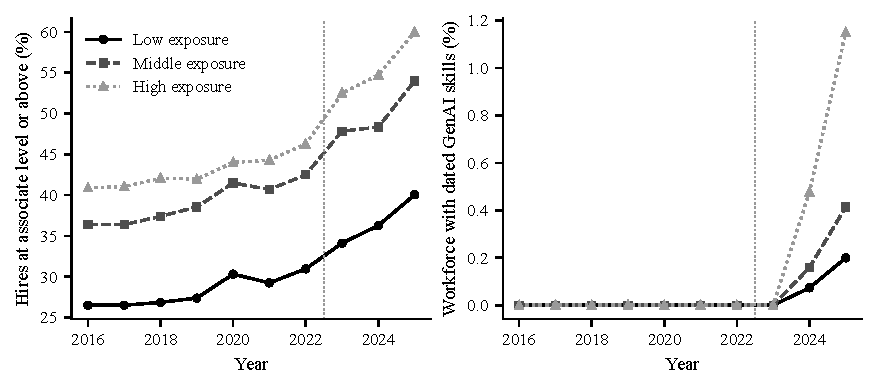
\includegraphics[width=\linewidth]{../figures/desc_event_time_means.pdf}
\caption{Raw means by exposure tercile: experienced-hire share (left) and workforce generative-AI adoption (right). The
dotted line marks the release of ChatGPT.}\label{fig:es}
\end{figure}
\begin{figure}[H]\centering
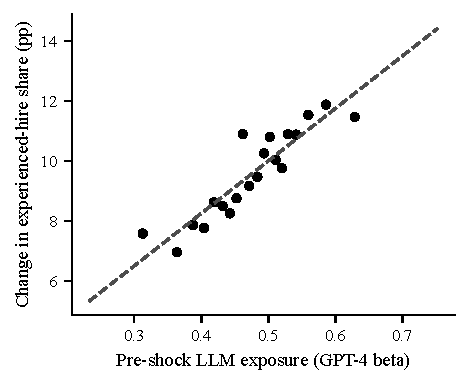
\includegraphics[width=0.55\linewidth]{../figures/desc_binscatter_change.pdf}
\caption{Bin scatter (20 bins) of each firm's post-minus-pre change in the experienced-hire share against its pre-shock LLM
exposure, with the OLS line.}
\end{figure}
\begin{figure}[H]\centering
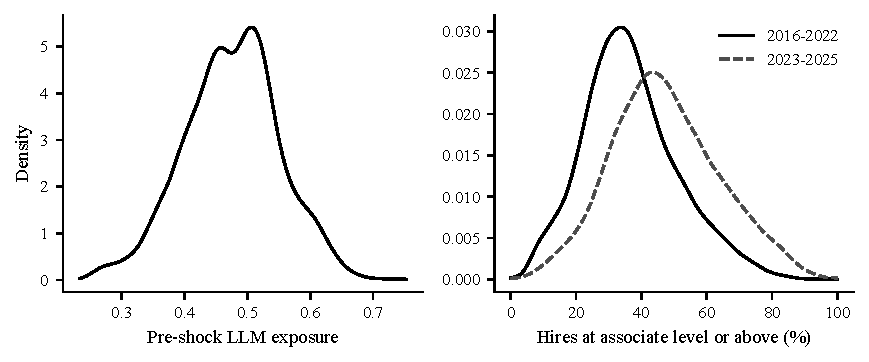
\includegraphics[width=\linewidth]{../figures/desc_densities.pdf}
\caption{Kernel densities of pre-shock exposure (left) and of the experienced-hire share before and after the shock (right).}
\end{figure}

%======================================================================
\section{Calibration results}\label{sec:calib}
%======================================================================
\IfFileExists{../tables/tab_procedures.tex}{\begin{table}[!htbp]\centering\footnotesize
\caption{Potemkin rates and search-adjusted inference}\label{tab:procedures}
\begin{tabular}{lrr}
\toprule
Procedure & Rate / $p$ & Interval / adjusted \\
\midrule
U (registered signs) & 26.5 & [23.8, 29.2] \\
U-free (signs rationalized) & 93.4 & [91.9, 94.9] \\
Bonferroni over models visited & 0.0 & [0.0, 0.0] \\
Specification curve (median t >= 1.96) & 3.3 & [2.2, 4.4] \\
NWC (loop-level p <= .05) & 5.0 & [3.6, 6.4] \\
Guard: split sample, one confirmation, Holm & 0.6 & [0.0, 1.3] \\
\midrule \multicolumn{3}{l}{\textit{Search-adjusted $p$-values for the real report}} \\
H1 (maximum $t$ over the search) & 0.001 &  \\
Package reported by loop U & 0.056 &  \\
Moderator Organizational age (log) (Type B, B=500) & 0.313 & Holm over ten: 1.000 \\
Moderator Digitizable work (Type B, B=500) & 0.046 & Holm over ten: 0.413 \\
Moderator Hierarchy shape (log ratio) (Type B, B=500) & 0.002 & Holm over ten: 0.020 \\
\bottomrule
\end{tabular}
\begin{minipage}{0.95\linewidth}\vspace{2pt}\scriptsize\textit{Notes.} Top panel: share (\%) of 1,000 Type A null worlds (LLM exposure permuted across firms within 2-digit NAICS sectors) in which the procedure reports H1 and three moderators all significant at the 5\% level with mixed signs; 95\% Monte Carlo intervals. Bottom panel: rank of the real statistic among the null-world statistics produced by the same loop (Theorem 1). Holm over ten: step-down adjustment over all ten registered moderators, the seven the loop did not report counted as $p=1$ (Table~\ref{tab:v_modreal}).\end{minipage}
\end{table}}{}

\paragraph{Reading the results.}
\begin{itemize}
\item \textbf{Null worlds are not quiet.} Across \Bnull Type~A worlds, H1 is nominally significant in \NullShareHoneSig\% of
the base specifications on average, although exposure has no firm-specific effect by construction. Sector-level co-movement,
which within-sector permutation preserves, is enough to generate large $t$-statistics under firm and year fixed effects.
The 95th percentile of the loop's maximum H1 $t$ in null worlds is \NullHoneQ.
\item \textbf{Potemkin rates.} The unguarded loop reports a full package in \PotemU\% of null worlds. Letting it
rationalize moderator signs raises this to \PotemFree\%.
\item \textbf{Search-adjusted inference.} The real data's maximum H1 $t$ (\HoneMaxT) exceeds every null world, and the
reported package has search-adjusted $p=\pNWCpkg$.
\end{itemize}

\paragraph{An ex post diagnostic for the moderators.} In Type~B worlds for digitizable work, the loop still selects the
\emph{permuted} moderator in most worlds. Permuting within sector $\times$ exposure-quintile strata preserves the moderator's
stratum-level association with exposure, so part of what the loop reads as moderation by digitizable work is heterogeneity of
the exposure effect across sectors and exposure levels. Consistent with this, adding exposure$^2\times$Post to the reported
package shrinks the digitizable-work interaction from $t=-4.40$ to $t=-2.95$, while the hierarchy-shape ($t=-5.21$) and
organizational-age ($t=2.30$) interactions are unchanged (\texttt{tables/expost\_nonlinearity.json}). This diagnostic was run
after the Type~B results were seen and is labelled accordingly.

\begin{figure}[H]\centering
\IfFileExists{../figures/fig5_planted.pdf}{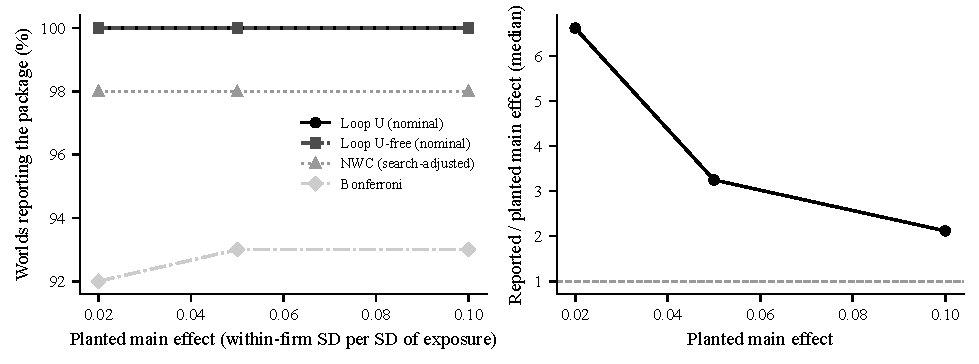
\includegraphics[width=\linewidth]{../figures/fig5_planted.pdf}}{}
\caption{Planted worlds: share of worlds in which each procedure reports the full package (left), and the median ratio of
the main effect reported by loop U to the planted effect (right). Planted moderators: 0.05 within-firm SD in their
registered directions.}\label{fig:planted}
\end{figure}
\begin{figure}[H]\centering
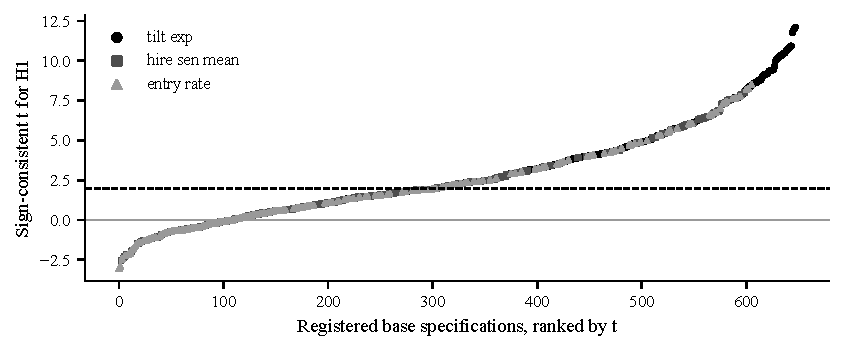
\includegraphics[width=\linewidth]{../figures/figA_spec_curve.pdf}
\caption{Specification curve: sign-consistent H1 $t$-statistics across the \NbaseSpecs registered base specifications, by
outcome proxy.}
\end{figure}

%======================================================================
\section{Monte Carlo evidence on synthetic twins}\label{sec:mc}
%======================================================================
\IfFileExists{../tables/tab_mc.tex}{\begin{table}[!htbp]\centering\footnotesize
\caption{Monte Carlo on synthetic twins: rejection rates (\%)}\label{tab:mc}
\begin{tabular}{p{6.2cm}rrrrrr}
\toprule
Scenario & $R$ & U & Bonferroni & Spec.\ curve & NWC package & NWC H1 \\
\midrule
Null (no effect; treatment exchangeable within sector) & 200 & 0.0 & 0.0 & 11.0 & 0.0 & 5.0 \\
Null, moderators chosen by peeking at outcomes (not replayed) & 300 & 0.0 & 0.0 & 10.0 & 0.0 & 10.3 \\
Null, the same peeking step replayed in every null world & 200 & 0.0 & 0.0 & 11.0 & 0.0 & 5.0 \\
No causal effect; unobserved trait drives both exposure and post-period drift & 50 & 0.0 & 0.0 & 94.0 & 4.0 & 90.0 \\
Planted effects (H1 0.10 SD; three moderators $\pm$0.06 SD) & 50 & 82.0 & 60.0 & 100.0 & 82.0 & 100.0 \\
\bottomrule
\end{tabular}
\begin{minipage}{0.95\linewidth}\vspace{2pt}\scriptsize\textit{Notes.} Each replication draws a synthetic twin (Section~\ref{sec:mc}), runs the reduced registered loop (12 base specifications and the 10-moderator search), and computes loop-level $p$-values from $B$ inner null worlds (within-sector permutation of exposure). Under the null, NWC rejection rates should not exceed 5\% up to Monte Carlo error; Theorem 1 does not cover the leakage and confounded scenarios, which show what the method cannot do.\end{minipage}
\end{table}}{}

\paragraph{What the Monte Carlo shows.}
\begin{itemize}
\item \textbf{Size.} Under the null, the loop-level test of the searched main effect rejects in \MCsizeNWC\% of replications,
consistent with Theorem~1 given Monte Carlo error. The specification-curve rule rejects in \MCsizeSpec\%: sector-level shocks
correlated with exposure make many specifications nominally significant.
\item \textbf{Proposal leakage.} Suppose the analyst peeks at the results, prunes the design space to the best-looking
specification, and only then registers it. The test then rejects in \MCsizeLeak\% of null replications. Replaying the
pruning inside every null world restores \MCsizeLeakReplay\%. This is the replayability principle in numbers.
\item \textbf{Confounding.} When an unobserved trait drives both exposure and post-period outcome drift, the test rejects
in \MCsizeConf\% of replications. Null-World Calibration prices search, not confounding. Section~\ref{sec:validity} maps
how the rejection rate grows with the strength of such a trait, and what restores size when the trait is observed.
\item \textbf{Power.} With planted effects, the package test rejects in \MCpowerNWC\% of replications and the main-effect test
in \MCpowerNWChOne\%.
\item \textbf{Twin versus real null worlds.} In the twin, the unguarded loop rarely assembles a full package under the null
(\MCsizeU\%), whereas it does so in \PotemU\% of real-data null worlds. Real organizational data carry moderator-linked
trends and heterogeneous shocks that a simple generative model omits. This is a reason to calibrate on null worlds built from
the real data rather than on simulations alone.
\end{itemize}

The synthetic twin is a generative model fitted to the analysis panel (\texttt{nullworld/synth.py}):
\begin{itemize}
\item a Gaussian copula over firm-level exposure, moderators, and pre-period covariates;
\item sectors drawn conditional on exposure quintile;
\item coverage patterns borrowed from real firms;
\item outcomes and controls built from firm effects, year effects, sector-year shocks, and AR(1) within-firm shocks.
\end{itemize}
\begin{sloppypar}
It reproduces means, between- and within-firm standard deviations, and the firm-level correlations among exposure and
moderators. It understates within-firm serial correlation (\nolinkurl{intermediate/08_twin_fidelity.csv}).
\end{sloppypar}

%======================================================================
\section{Validity diagnostics}\label{sec:validity}
%======================================================================
This section examines the conditions under which the calibration is valid: who took which decision, what happens
when exposure is not exchangeable within sector, what the moderator tests and their $p$-values measure (including the
familywise correction over all ten registered candidates), and what replay costs. The analyses were added after the main
results were seen (20 October 2026). They are diagnostics: they test whether the calibration's conditions hold and what its
$p$-values measure, and no claim is upgraded on their strength alone. Scripts: \texttt{scripts/22}--\texttt{27}; all numbers
in \texttt{tables/validity.json} and \texttt{tables/benchmark.json}.

\subsection{Who decided what}
% Decision ledger of the prototype (who decided what, when, and whether it is replayed).
% Sources: registry/design_space.yaml (field `authoring`), README.md (AI use), intermediate/00_design_decisions.md.
\begin{table}[!htbp]\centering\footnotesize
\caption{Who took which research decision in the prototype, and how calibration treats it}\label{tab:v_ledger}
\begin{tabular}{>{\raggedright\arraybackslash}p{4.5cm}>{\raggedright\arraybackslash}p{3.3cm}>{\raggedright\arraybackslash}p{2.6cm}>{\raggedright\arraybackslash}p{4.2cm}}
\toprule
Decision & Proposed / taken by & When & Treatment in calibration \\
\midrule
Research question, testbed, fit with the call & Authors & Before data access & Fixed; outside the loop \\
Constructs and proxies (3 outcomes, 3 exposures), controls, fixed effects, samples, transforms, clustering & AI agent, from the literature; approved by the authors & Before any outcome (registry hashed 29~Sep~2026, 04:19) & Frozen and hashed: a non-replayable input that cannot depend on outcomes \\
Ten moderators with signs and mechanisms; H1 mechanism and rival & AI agent, from the literature; approved by the authors & Before any outcome & Frozen and hashed \\
Search policies U and U-free, package statistic, stopping rule & Specified in the registry; coded by the AI agent & Before any outcome & Code: replayed identically in every world \\
Data assembly and measurement audits (skill dictionary, role crosswalk, linkage) & AI agent; reviewed by the authors & Before any outcome & Fixed code; audits reported \\
Run-time choices: which specification next, which moderators to keep, which triples, when to stop, which signs (U-free) & The coded policy & After data access & Replayed in every null, moderator, and planted world \\
Ex post identification checks (trend break, 2019+ window, exposure$^2$ diagnostic) & Authors with the AI agent & After outcomes were seen & Not priced; labelled ex post \\
\textit{Stage 2:} run-time choices taken by a live LLM agent & LLM agent (open weights, deterministic decoding) & After data access & Each call logged and re-issued in every world \\
\bottomrule
\end{tabular}
\begin{minipage}{0.97\linewidth}\vspace{2pt}\scriptsize\textit{Notes.} Reconstructed from \texttt{registry/design\_space.yaml}
(field \texttt{authoring}), the AI-use statement in \texttt{README.md}, and the dated entries of
\texttt{intermediate/00\_design\_decisions.md}. The AI agent works under the authors' direction.\end{minipage}
\end{table}

The AI agent's decisions in the prototype were taken before outcomes were computed, and they are frozen in the registry
or the code. All run-time choices are code and are replayed. Policies U and U-free are benchmarks that bracket an agent's
search; they are not models of agent behaviour. Figure~\ref{fig:budget} shows how their Potemkin rates grow with the number
of models a loop may fit before reporting.
\begin{figure}[H]\centering
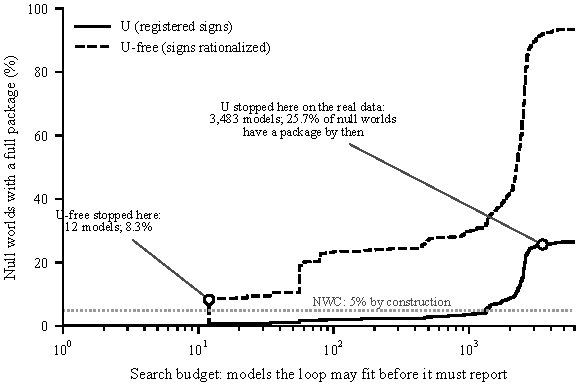
\includegraphics[width=0.6\linewidth]{../figures/fig10_budget.pdf}
\caption{Share of the \Bnull Type~A null worlds in which each policy has reported a fully significant package within a given
number of models (search budget). Markers: where each policy stopped on the real data.}\label{fig:budget}
\end{figure}

\subsection{When exposure is not exchangeable within sector}
Within NAICS-2 sectors, exposure is correlated with several firm traits: \VcorrExpRem with digitizable work, \VcorrExpPyr with
hierarchy shape, \VcorrExpAI with pre-period AI talent, and \VcorrExpGrowth with pre-period hiring growth. Type~A worlds break these links.
Table~\ref{tab:v_exch} and Figure~\ref{fig:exch} measure the consequence on synthetic twins with no exposure effect. A trait
$u$ with within-sector correlation $\rho$ with exposure shifts outcomes either in levels or after the shock.
\begin{itemize}
\item \textbf{Level-only traits are harmless.} Firm effects absorb them (\VExLevel\% rejections; \VExNull\% with no trait).
\item \textbf{Post-shock traits are confounders.} Rejections rise quickly with the spurious effect they induce:
\VExNWCTwoFive\% when it is \VExSpurTwoFive\% of the real H1 estimate, \VExNWCFourFive\% at \VExSpurFourFive\%, and
\VExNWCSixTen\% at \VExSpurSixTen\%. A correctly sized test of an association detects a confounded association as readily as a
real one: calibration prices search, not confounding. Nominal tests give no protection either. One pre-specified regression
already rejects in \VExSingleNull\% of null twins, because sector shocks correlated with exposure fool its reference
distribution, and it rises with confounding too.
\item \textbf{Observed traits have a remedy.} Strata on the trait's quintile help only partly (up to \VExStratMax\%). Worlds
that preserve exposure's projection on the trait hold size in all \VExNcells settings (at most \VExCovMax\%).
\end{itemize}
On the real data (Table~\ref{tab:v_covA}), worlds that preserve exposure's within-sector projection on twelve predetermined
traits give $p\le\VcovAph$ for H1 and $p=\VcovApkg$ for the package. The unguarded loop's Potemkin rate rises to
\VcovAPotU\%: exposure-correlated traits give a searching loop more ways to assemble a package.
\begin{table}[!htbp]\centering\footnotesize
\caption{Monte Carlo: rejection rates (\%) when exposure is not exchangeable within sector}\label{tab:v_exch}
\setlength{\tabcolsep}{4.5pt}\begin{tabular}{lrrrrrrrr}
\toprule
 & & & Spurious & \multicolumn{3}{c}{NWC worlds} & \multicolumn{2}{c}{Nominal} \\
\cmidrule(lr){5-7}\cmidrule(lr){8-9}
Trait channel & $\rho$ & $\delta$ & effect (\%) & within sector & strata on $u$ & $u$-preserving & one regression & naive loop \\
\midrule
level only & 0.6 & 1 & 1 & 6.0 & 6.5 & 6.0 & 17.0 & 20.5 \\
none (null) & 0.0 & 0 & 1 & 6.5 & 5.5 & 6.0 & 17.0 & 19.5 \\
post-shock shift & 0.2 & 0.025 & 3 & 11.5 & 6.0 & 6.5 & 20.0 & 23.5 \\
post-shock shift & 0.2 & 0.05 & 5 & 19.5 & 6.0 & 7.0 & 25.0 & 30.0 \\
post-shock shift & 0.2 & 0.1 & 9 & 39.5 & 9.0 & 6.0 & 35.0 & 42.0 \\
post-shock shift & 0.2 & 0.2 & 18 & 87.0 & 12.0 & 5.5 & 58.5 & 61.5 \\
post-shock shift & 0.4 & 0.025 & 5 & 20.0 & 7.0 & 6.0 & 25.5 & 30.5 \\
post-shock shift & 0.4 & 0.05 & 9 & 43.0 & 8.0 & 7.0 & 35.0 & 43.0 \\
post-shock shift & 0.4 & 0.1 & 18 & 87.5 & 14.5 & 6.0 & 61.5 & 63.0 \\
post-shock shift & 0.4 & 0.2 & 34 & 100.0 & 22.0 & 5.5 & 93.5 & 96.0 \\
post-shock shift & 0.6 & 0.025 & 7 & 29.0 & 9.5 & 5.5 & 30.5 & 35.5 \\
post-shock shift & 0.6 & 0.05 & 14 & 70.0 & 12.5 & 7.5 & 48.0 & 52.5 \\
post-shock shift & 0.6 & 0.1 & 26 & 100.0 & 19.5 & 5.5 & 84.5 & 87.0 \\
post-shock shift & 0.6 & 0.2 & 51 & 100.0 & 45.0 & 4.5 & 100.0 & 100.0 \\
\bottomrule
\end{tabular}
\begin{minipage}{0.97\linewidth}\vspace{2pt}\scriptsize\textit{Notes.} $R=200$ synthetic twins per row, $B=99$ null worlds per twin; Monte Carlo standard error about 1.5 points at 5\%. Exposure has no effect. A firm trait $u$ with within-sector correlation $\rho$ with exposure shifts the outcome either in levels (1 between-firm SD) or after the shock ($\delta$ within-firm SDs). Spurious effect: the mean estimate of the pre-specified regression as a share of the real H1 estimate. NWC: within-sector permutation (the application's Type A worlds); strata on $u$: within sector $\times$ quintile of $u$; $u$-preserving: exposure = projection on (sector, $u$) + permuted residual.\end{minipage}
\end{table}
\begin{figure}[H]\centering
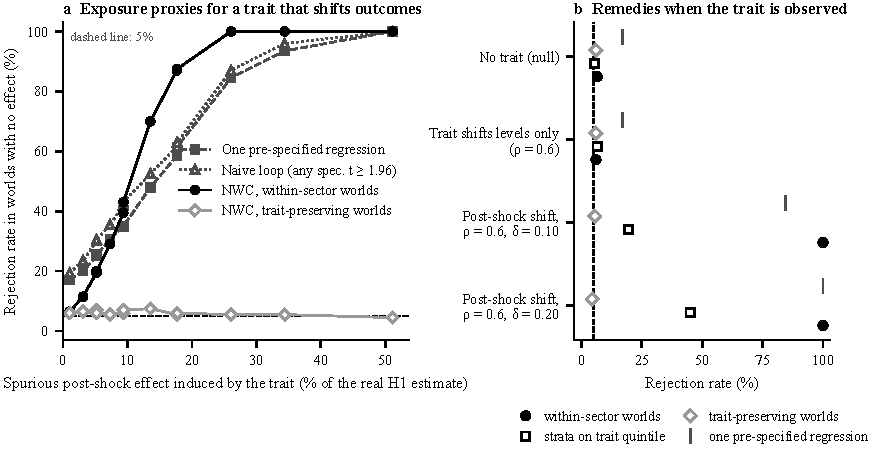
\includegraphics[width=\linewidth]{../figures/fig7_exchangeability.pdf}
\caption{Synthetic twins with no exposure effect and a trait correlated with exposure within sector. (a)~Rejection rates
against the spurious effect the trait induces (as a share of the real H1 estimate). (b)~The null, a level-only trait, and two
post-shock cells under four procedures.}\label{fig:exch}
\end{figure}
\begin{table}[!htbp]\centering\footnotesize
\caption{Real data: Type A worlds versus covariate-preserving worlds}\label{tab:v_covA}
\begin{tabular}{lrr}
\toprule
 & Type A (within sector) & Covariate-preserving \\
\midrule
Worlds & 1,000 & 1,000 \\
Largest null H1 $t$: median / 95th pct.\ / max & 7.4 / 8.6 / 9.8 & 7.2 / 8.0 / 9.3 \\
Search-adjusted $p$, H1 (real $t=12.1$) & 0.001 & 0.001 \\
Search-adjusted $p$, full package & 0.056 & 0.137 \\
Potemkin rate, U (\%) & 26.5 & 40.3 \\
Potemkin rate, U-free (\%) & 93.4 & 100.0 \\
\bottomrule
\end{tabular}
\begin{minipage}{0.97\linewidth}\vspace{2pt}\scriptsize\textit{Notes.} Covariate-preserving worlds keep each exposure proxy's within-sector projection on twelve predetermined traits (the ten moderators, pre-period size and hiring growth; within-sector $R^2$ 53\% for the main proxy) and permute only the residual within sector, so trait-driven outcome trends are present in every null world.\end{minipage}
\end{table}

\subsection{Moderator nulls and what the moderator \texorpdfstring{$p$}{p} measures}
Table~\ref{tab:v_modmc} and Figure~\ref{fig:mod} report the size of three moderator-world constructions when the target's
true interaction is zero. The target is given its own post-shock trend, a correlated moderator with a true interaction, and a
concave exposure effect, all with adversarial signs. The moderator's own trend is harmless (\VMmPermFixTrend\% rejections
under permutation), because every moderator model contains $M_k\times$Post. A correlated moderator with a real interaction
and a concave exposure effect are not: permutation rejects a zero interaction in \VMmPermFixProxy\% and \VMmPermFixNonlin\%
of samples, and in \VMmPermFixAll\% with all three structures. Conditional permutation holds size in every scenario
(\VMmResFixAll\% with all three). Null-model worlds are valid but conservative (\VMmFLFixAll\%); their $p$-values cluster near
0.5. Table~\ref{tab:v_modreal} and Figure~\ref{fig:sel} give the real-data
$p$-values by construction and statistic, with the familywise corrections over the ten registered candidates. With all ten
moderators permuted, the loop still reports a fully significant package in \VJointSuccess\% of the \VBjoint joint worlds. Much
of what a loop reads as moderation in these data is the heterogeneity of a strong main effect.
\begin{table}[!htbp]\centering\footnotesize
\caption{Monte Carlo: rejection rates (\%) of moderator tests when the true interaction is zero}\label{tab:v_modmc}
\setlength{\tabcolsep}{4.5pt}\begin{tabular}{lrrrrrrrr}
\toprule
 & \multicolumn{4}{c}{With search ($S^{\text{free}}$)} & \multicolumn{4}{c}{One specification ($S^{\text{fix}}$)} \\
\cmidrule(lr){2-5}\cmidrule(lr){6-9}
Scenario & Nominal & Perm. & Cond. & Null m. & Nominal & Perm. & Cond. & Null m. \\
\midrule
No other structure & 4.5 & 4.0 & 7.0 & 0.5 & 2.5 & 4.0 & 5.0 & 0.5 \\
Own post-shock trend of $M_k$ & 3.5 & 1.5 & 5.5 & 1.0 & 2.5 & 2.0 & 5.0 & 0.5 \\
Correlated moderator, true interaction & 96.0 & 65.5 & 5.0 & 0.5 & 95.0 & 67.5 & 5.0 & 0.5 \\
Concave exposure effect & 96.5 & 35.5 & 5.5 & 0.5 & 96.0 & 35.0 & 6.0 & 0.5 \\
All three & 96.5 & 91.5 & 4.5 & 0.5 & 100.0 & 95.0 & 4.5 & 0.5 \\
\bottomrule
\end{tabular}
\begin{minipage}{0.97\linewidth}\vspace{2pt}\scriptsize\textit{Notes.} $R=200$ synthetic twins per row with a planted main effect (0.10 within-firm SD), $B=59$ worlds per construction. Target: hierarchy shape, whose true interaction is zero. Own trend: $+0.10$ SD $\times M_k\times$Post; correlated moderator: digitizable work ($r=-0.60$ with $M_k$) with interaction $-0.06$ SD; concave exposure: $-0.05$ SD $\times(E^2-1)\times$Post. Signs are adversarial: the leakage runs in $M_k$'s registered direction. Perm.: within sector $\times$ exposure quintile (Type B); Cond.: conditional permutation, only the part of $M_k$ not explained by sector, exposure, exposure$^2$ and the other nine moderators is permuted; Null m.: null-model Freedman--Lane worlds with residuals sign-flipped by firm.\end{minipage}
\end{table}
\begin{figure}[H]\centering
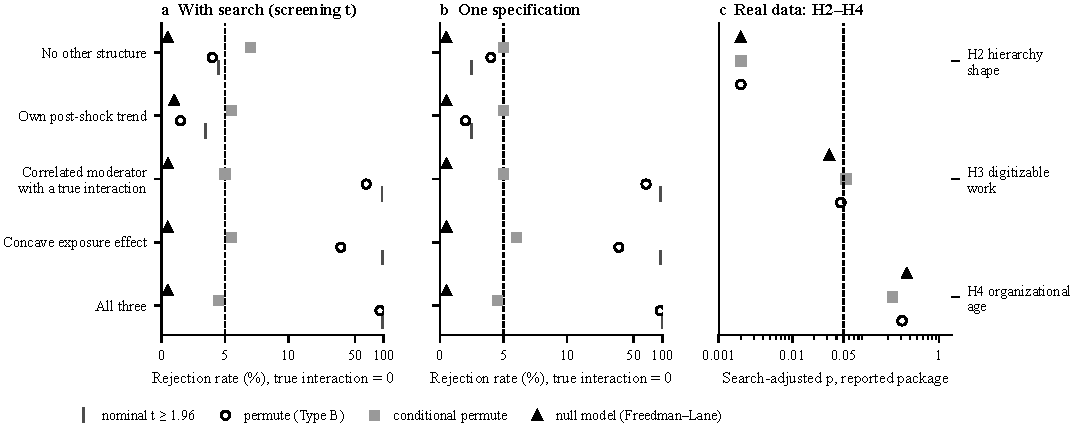
\includegraphics[width=\linewidth]{../figures/fig8_moderator_worlds.pdf}
\caption{Moderator tests when the true interaction is zero: Monte Carlo rejection rates by construction (a,\,b), and the
real-data $p$-values of H2--H4 under the three constructions (c).}\label{fig:mod}
\end{figure}
\begin{table}[!htbp]\centering\footnotesize
\caption{Search-adjusted $p$-values of the reported moderators, by world construction and statistic}\label{tab:v_modreal}
\setlength{\tabcolsep}{4pt}\begin{tabular}{>{\raggedright\arraybackslash}p{2.6cm}>{\raggedright\arraybackslash}p{5.3cm}rrr}
\toprule
 & & H2 hierarchy & H3 digitizable & H4 organiz. \\
 & & shape & work & age \\
\midrule
\multicolumn{2}{l}{Observed $t$ in the package ($S^{\text{sel}}=S^{\text{fix}}$)} & 5.57 & 4.57 & 2.60 \\
\multicolumn{2}{l}{Observed largest screening $t$ ($S^{\text{free}}$)} & 6.27 & 14.84 & 6.99 \\
\multicolumn{2}{l}{Share of permuted worlds reporting the moderator} & 0.4\% & 92.8\% & 76.6\% \\
\midrule
Permute (Type B) & $S^{\text{sel}}$ (reported package) & 0.002 & 0.046 & 0.313 \\
 & $S^{\text{free}}$ (screening, all worlds) & 0.002 & 0.601 & 0.002 \\
 & $S^{\text{fix}}$ (reported specification) & 0.002 & 0.018 & 0.022 \\
 & Holm over ten candidates ($S^{\text{sel}}$) & 0.020 & 0.413 & 1.000 \\
\addlinespace
Conditional permute & $S^{\text{sel}}$ (reported package) & 0.002 & 0.054 & 0.234 \\
 & $S^{\text{free}}$ (screening, all worlds) & 0.002 & 0.337 & 0.004 \\
 & $S^{\text{fix}}$ (reported specification) & 0.002 & 0.058 & 0.228 \\
 & Holm over ten candidates ($S^{\text{sel}}$) & 0.020 & 0.485 & 1.000 \\
\addlinespace
Null model (Freedman--Lane) & $S^{\text{sel}}$ (reported package) & 0.002 & 0.032 & 0.365 \\
 & $S^{\text{free}}$ (screening, all worlds) & 0.002 & 0.693 & 0.220 \\
 & $S^{\text{fix}}$ (reported specification) & 0.002 & 0.184 & 0.146 \\
 & Holm over ten candidates ($S^{\text{sel}}$) & 0.020 & 0.287 & 1.000 \\
\addlinespace
Joint (all ten permuted) & max-$T$ step-down (planned), $S^{\text{sel}}$ & 0.171 & 0.279 & 0.651 \\
 & min-$P$ step-down, $S^{\text{sel}}$ & 0.010 & 0.678 & 0.678 \\
 & min-$P$ step-down, $S^{\text{free}}$ (all ten tested) & 0.009 & 0.979 & 0.009 \\
\bottomrule
\end{tabular}
\begin{minipage}{0.97\linewidth}\vspace{2pt}\scriptsize\textit{Notes.} $p=(1+\#\{b: S_b\ge S_{\text{obs}}\})/(B+1)$ with $B=500$ worlds per moderator and construction ($B=1,000$ joint worlds); the smallest attainable $p$ is 0.002 (0.001 for joint worlds). $S^{\text{sel}}$ is $-\infty$ when the loop does not report the moderator, so its $p$ combines strength and selection. Holm over ten treats the seven unreported candidates as $p=1$.\end{minipage}
\end{table}
\begin{figure}[H]\centering
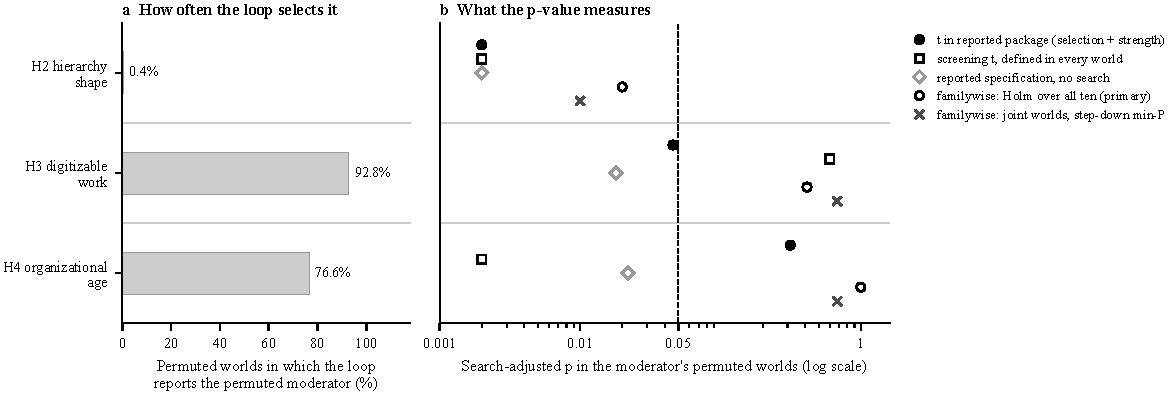
\includegraphics[width=\linewidth]{../figures/fig9_selection.pdf}
\caption{What the moderator $p$-value measures: the share of permuted worlds in which the loop reports the permuted
moderator (a), and the $p$-values of the three statistics with the familywise adjustments over ten candidates (b).}\label{fig:sel}
\end{figure}

\subsection{What replay costs}
One full replay of the registered loop (both policies, the whole design space, about \VFitsWorld model fits) takes
\VSecWorld seconds with the \texttt{nullworld} engine on the real panel. Refitting the same models with \texttt{pyfixest}
takes about \VPyfixestModel seconds each, or \VPyfixestWorld seconds per world, roughly \VSpeedup times longer. At
\Bnull worlds, that is the difference between under an hour and several days (\texttt{scripts/27\_benchmark.py}).

%======================================================================
\section{The registry}\label{sec:registry}
%======================================================================
\begin{sloppypar}
The registry below was frozen and hashed (SHA-256 prefix \texttt{\RegistryHash}, \RegistryTime) before any outcome was
computed. Deviations after freezing are listed in the design log (\nolinkurl{intermediate/00_design_decisions.md}):
\end{sloppypar}
\begin{itemize}
\item the handling of missing moderators, decided before outcomes were seen;
\item the adoption variable, decided before any IV estimate;
\item three ex post identification checks;
\item a reduced planted-world design, for compute reasons.
\end{itemize}
The listing omits the file's four-line \texttt{authoring} note (lines 11--14); the hash refers to the complete file in
the repository.
\lstinputlisting[linerange={1-10,15-99999}]{../registry/design_space.yaml}

%======================================================================
\section{Repository and reproduction}\label{sec:repo}
%======================================================================
The research artifact submitted with this appendix is the public repository \url{https://github.com/LLMPlus-ai/potemkin-findings}. Its numbered scripts write every number,
table, and figure, and each records its inputs and outputs in its header.
\begingroup\raggedright
\begin{itemize}
\item \texttt{registry/} holds the frozen design space and its SHA-256 hash; every run of the loop verifies the hash first.
\item \texttt{nullworld/} is the reusable package: fixed-effects engine, replayable loop, world generators, randomization
inference, synthetic twin, and registry grammar (Section~\ref{sec:loop}).
\item \texttt{scripts/01}--\texttt{07} build the data from the licensed sources (DuckDB, memory capped at 4~GB);
\texttt{scripts/08} fits and releases the synthetic twin.
\item \texttt{scripts/09}--\texttt{14} estimate the testbed, run the loop on the real data, generate the null, guard, and
planted worlds, run the Monte Carlo study, and aggregate Potemkin rates and search-adjusted $p$-values.
\item \texttt{scripts/22}--\texttt{27} produce the validity diagnostics of Section~\ref{sec:validity} and the cost benchmark.
\item \texttt{scripts/12}, \texttt{15}, \texttt{16}, \texttt{19}--\texttt{21}, and \texttt{26} write the figures and
tables; \texttt{scripts/17} and \texttt{25} write every number cited in the text as a macro.
\item \texttt{scripts/18} verifies every reference against Crossref (\texttt{literature/citation\_audit.csv});
\texttt{scripts/28} recomputes the cited validity numbers independently from the stored worlds;
\texttt{scripts/90}--\texttt{92} validate the engine against \texttt{pyfixest}.
\item \texttt{intermediate/} stores the output of every world (Type~A, Type~B, joint, trait-preserving, conditional,
rebuilt-outcome, guard, and planted) and every Monte Carlo replication.
\end{itemize}
\endgroup
\paragraph{Without licensed data.} The Revelio, Compustat, and I/B/E/S extracts cannot be redistributed and are not in
the repository. With \texttt{NULLWORLD\_DATA=synthetic}, the loop and all null worlds (\texttt{scripts/10}--\texttt{11})
run on the synthetic twin in \texttt{synthetic/}. The Monte Carlo studies (\texttt{scripts/13}, \texttt{23},
\texttt{24}) simulate their own twins, and the figure and table scripts read only the stored outputs. The scripts that
read the licensed data directly (01--09, 12, 14, 22, 25, 27; script 08 to fit the twin) document every field they use, so
licensees can regenerate every number.

\begin{thebibliography}{99}
\setlength{\itemsep}{1pt}\small
\bibitem[Autor et al.(2003)]{autor2003skill} Autor DH, Levy F, Murnane RJ (2003) The skill content of recent technological change: An empirical exploration. \textit{Quart. J. Econom.} 118(4):1279--1333.
\bibitem[Brynjolfsson et al.(2025)]{brynjolfsson2025generative} Brynjolfsson E, Li D, Raymond L (2025) Generative AI at work. \textit{Quart. J. Econom.} 140(2):889--942.
\bibitem[Cameron et al.(2008)]{cameron2008bootstrap} Cameron AC, Gelbach JB, Miller DL (2008) Bootstrap-based improvements for inference with clustered errors. \textit{Rev. Econom. Statist.} 90(3):414--427.
\bibitem[Dell'Acqua et al.(2026)]{dellacqua2026navigating} Dell'Acqua F, McFowland E III, Mollick E, Lifshitz H, Kellogg KC, Rajendran S, Krayer L, Candelon F, Lakhani KR (2026) Navigating the jagged technological frontier: Field experimental evidence of the effects of artificial intelligence on knowledge worker productivity and quality. \textit{Organ. Sci.} 37(2):403--423.
\bibitem[Eloundou et al.(2024)]{eloundou2024gpts} Eloundou T, Manning S, Mishkin P, Rock D (2024) GPTs are GPTs: Labor market impact potential of LLMs. \textit{Science} 384(6702):1306--1308.
\bibitem[Felten et al.(2021)]{felten2021occupational} Felten E, Raj M, Seamans R (2021) Occupational, industry, and geographic exposure to artificial intelligence: A novel dataset and its potential uses. \textit{Strategic Management J.} 42(12):2195--2217.
\bibitem[Felten et al.(2023)]{felten2023language} Felten E, Raj M, Seamans R (2023) How will language modelers like ChatGPT affect occupations and industries?. Preprint, arXiv:2303.01157.
\bibitem[Freedman and Lane(1983)]{freedman1983nonstochastic} Freedman D, Lane D (1983) A nonstochastic interpretation of reported significance levels. \textit{J. Bus. Econom. Statist.} 1(4):292--298.
\bibitem[Garicano(2000)]{garicano2000hierarchies} Garicano L (2000) Hierarchies and the organization of knowledge in production. \textit{J. Political Econom.} 108(5):874--904.
\bibitem[Gaure(2013)]{gaure2013ols} Gaure S (2013) OLS with multiple high dimensional category variables. \textit{Comput. Statist. Data Anal.} 66:8--18.
\bibitem[Hannan and Freeman(1984)]{hannan1984structural} Hannan MT, Freeman J (1984) Structural inertia and organizational change. \textit{Amer. Sociol. Rev.} 49(2):149--164.
\bibitem[Hansen(2005)]{hansen2005test} Hansen PR (2005) A test for superior predictive ability. \textit{J. Bus. Econom. Statist.} 23(4):365--380.
\bibitem[Hemerik and Goeman(2018)]{hemerik2018exact} Hemerik J, Goeman J (2018) Exact testing with random permutations. \textit{TEST} 27(4):811--825.
\bibitem[Lehmann and Romano(2022)]{lehmann2022testing} Lehmann EL, Romano JP (2022) \textit{Testing Statistical Hypotheses, 4th ed.} (Springer, Cham).
\bibitem[Levinthal and March(1993)]{levinthal1993myopia} Levinthal DA, March JG (1993) The myopia of learning. \textit{Strategic Management J.} 14(S2):95--112.
\bibitem[March(1991)]{march1991exploration} March JG (1991) Exploration and exploitation in organizational learning. \textit{Organ. Sci.} 2(1):71--87.
\bibitem[Noy and Zhang(2023)]{noy2023experimental} Noy S, Zhang W (2023) Experimental evidence on the productivity effects of generative artificial intelligence. \textit{Science} 381(6654):187--192.
\bibitem[Romano and Wolf(2005)]{romano2005stepwise} Romano JP, Wolf M (2005) Stepwise multiple testing as formalized data snooping. \textit{Econometrica} 73(4):1237--1282.
\bibitem[S{\o}rensen and Stuart(2000)]{sorensen2000aging} S{\o}rensen JB, Stuart TE (2000) Aging, obsolescence, and organizational innovation. \textit{Admin. Sci. Quart.} 45(1):81--112.
\bibitem[Westfall and Young(1993)]{westfall1993resampling} Westfall PH, Young SS (1993) \textit{Resampling-Based Multiple Testing: Examples and Methods for p-Value Adjustment} (Wiley, New York).
\bibitem[White(2000)]{white2000reality} White H (2000) A reality check for data snooping. \textit{Econometrica} 68(5):1097--1126.
\bibitem[Winkler et al.(2014)]{winkler2014permutation} Winkler AM, Ridgway GR, Webster MA, Smith SM, Nichols TE (2014) Permutation inference for the general linear model. \textit{NeuroImage} 92:381--397.
\end{thebibliography}

\end{document}
